\documentclass[iop]{emulateapj-rtx4}


%\documentclass[12pt]{article}
%\pdfpagewidth 8.5in
%\pdfpageheight 11in 
%\setlength\topmargin{0in}
%\setlength\headheight{0in}
%\setlength\headsep{0in}
%\setlength\textheight{9in}
%\setlength\textwidth{6.5in}
%\setlength\oddsidemargin{0in}
%\setlength\evensidemargin{0in}

\usepackage{graphicx}
\usepackage{amssymb}

%\usepackage{multicol}
%\usepackage{sidecap}
%\usepackage{ragged2e}

%\usepackage{caption}
%\usepackage{subcaption}

\usepackage{wrapfig}
\usepackage{setspace}
\usepackage{subfigure}
\usepackage{mathtools}


%\newcommand{\rms}[1]{\langle #1 \rangle}
%\renewcommand{\baselinestretch}{1.5}
%\renewcommand{\thefootnote}{\roman{footnote}}

\graphicspath{{paper_figures3//}}


\frenchspacing

\begin{document}

%\onehalfspacing

%\title{A Dichotomy in the Relative Velocity of Ly$\alpha$ Absorption in Nearby Galaxy Halos}
\title{Matching Ly$\alpha$ Absorption to Nearby Galaxy Halos with a Likelihood-based Method}

\author{David M. French, Bart P. Wakker}
\affil{Department of Astronomy, University of Wisconsin - Madison}

%\affil{Department of Astronomy, University of Wisconsin - Madison; frenchd@astro.wisc.edu}


\begin{abstract}

We present initial results from an ongoing large-scale study of the circumgalactic medium in the nearby Universe ($cz \leq 10,000$ km/s), using archival Cosmic Origins Spectrograph (COS) and Space Telescope Imaging Spectrograph (STIS) spectra of background QSOs. This initial sample contains 35 sight lines, yielding 175 Ly$\alpha$ systems, 41 of which we have paired with nearby galaxies. We introduce a likelihood parameter to quantitatively predict the galaxy responsible for measured absorption in a reproducible way. Results from this sample suggest an anti-correlation between Ly$\alpha$ equivalent width ($W$) and impact parameter ($\rho$) when we normalize by galaxy virial radius ($R_{vir}$). Absorption is detected in excess near galaxies with inclination $>60^\circ$, and near $\rho= 1.2 R_{vir}$. We also detect a dichotomy in the equivalent widths of absorption systems around $\Delta v = v_{galaxy} - v_{gas}$, with positive $\Delta v$ absorption median $W$ = $343 \pm 10$ m\AA, and negative $\Delta v$  absorption median $W$ = $124 \pm 9$ m\AA. 

%This $W$ difference is significant at a greater than $99\%$ confidence limit. We also find a positive correlation between absorber-galaxy impact parameter and galaxy $R_{vir}$, a preference for absorption around highly inclined galaxies, but little evidence of azimuthal dependence.


%Galaxies must accrete gas from the intergalactic medium (IGM) in order to sustain star formation at observed levels. In order to understand this complex process, and how it influences galaxy evolution, it is necessary to understand the physical conditions and distribution of the gas around galaxies, known as the circumgalactic medium (CGM). For my thesis, I propose to use archival spectra of bright background QSOs taken by the Cosmic Origins Spectrograph (COS) on the Hubble Space Telescope (HST) to directly probe the CGM of galaxies in the nearby Universe. I will supplement this spectral data with observations of these galaxies taken by the WIYN and SALT telescopes. This proposed program will be the largest and most statistically significant survey of the local CGM to date.

\end{abstract}
\keywords{IGM, CGM, galaxies}


%\section{THINGS I STILL NEED}
%
%- galaxy table completeness plot
%- breakdown of systems into single galaxy (certain), multiple galaxies (probable), multiple galaxies (ambiguous)
%- mean Lstar for associated galaxies of each type


\section{Introduction}

It is well known that galaxies must continue to accrete gas throughout their lifetimes in order to sustain observed levels of star formation (e.g. Erb 2008, Putman et al. 2009b). This additional gas must come from the diffuse intergalactic medium (IGM), where the majority of the baryons in the universe reside (Penton et al. 2002, 2004; Lehner et al. 2007; Danforth $\&$ Shull 2008; Shull et al. 2012). How exactly this IGM gas eventually falls into the halos and disks of galaxies is still highly uncertain, as observational constraints are hard to come by. Because of the diffuse nature of IGM gas, it is most readily and sensitively detected as absorption in the spectra of background active galactic nuclei (AGN). The advent of the sensitive UV spectrographs STIS and COS on the Hubble Space Telescope (HST) has provided a wealth of information on the properties and distribution of both the ions of heavy elements as well as the Lyman series of neutral H\,{\sc i} gas around galaxies. 

Individual concentrations of gas along a given sightline imprint absorption lines on the spectrum in the direction of the QSO. The metal lines trace the star formation history within the intervening gas, and neutral hydrogen lines (Ly$\alpha$) indicate both the location and velocities of outflowing gas as well as the presence of fuel for future star formation. Numerous studies using these observations have shown that many Ly$\alpha$ absorbers trace individual galaxy halos (e.g. Wakker $\&$ Savage 2009, Danforth et al. 2014, Stocke et al. 2013 $\&$ 2014, Liang et al 2014, Lanzetta et al 1995, Chen et al. 1998, 2001a, Tripp et al. 1998, Steidel et al. 2010, Prochaska et al. 2011, Thom et al 2012, Tumlinson et al. 2011 $\&$ 2013). 


%It is well known now that galaxies must continue to accrete gas throughout their lifetimes in order to sustain observed levels of star formation (e.g., see Erb 2008, Putman et al. 2009b). This additional gas comes from the diffuse intergalactic medium (IGM), where the majority of the baryons in the universe reside. In order to understand the life cycle of this gas and its effect on the evolution of nearby galaxies, it is necessary to understand its physical properties such as densities, temperatures, motions, and its interactions with the galaxies. This can be accomplished by analyzing lines of sight toward background QSOs.

%The current standard model of structure formation is given by $\Lambda$CDM cosmology, which predicts the hierarchical growth of large scale structures seeded by initial fluctuations in the dark matter background. In this picture, both galaxies and neutral H\,{\sc i} follow the same underlying density profile. Wakker et al. (2015, submitted) have provided some observational evidence for this, showing that Ly$\alpha$ absorption strength traces the large-scale distribution of galaxies in a Cosmic Web filament. In addition, numerous previous studies have shown that Ly$\alpha$ absorbers also trace individual galaxy halos (e.g. Wakker $\&$ Savage 2009, Danforth et al. 2014, Stocke et al. 2013, Liang et al 2014, Lanzetta et al 1995, Chen et al. 1998, 2001a, Tripp et al. 1998, Steidel et al. 2010, Prochaska et al. 2011, Thom et al 2012). 


Some recent studies find that about half of Ly$\alpha$ absorbers lie within galaxy haloes, at impact parameters $\rho<350$ kpc (C\^{o}t\'{e} et al. 2005, Prochaska et al. 2006). In addition, Wakker $\&$ Savage (2009) find that an absorber lies within 400 kpc and 400 km/s for $90$\%$ of galaxies brighter than 0.1L_{\**}$, and all galaxies have a Ly$\alpha$ absorber within 1.5 Mpc. Higher redshift studies, such as Rudie et al. (2012) at $2<z<3$, find evidence for an elevated density of absorbers up to 2 Mpc from galaxies. Wakker $\&$ Savage (2009) also confirmed a previously suggested correlation between Ly$\alpha$ absorption linewidth and impact parameter $\rho$, observing that the broadest lines (FWHM $>$150 km/s) are only seen within 350 kpc of a galaxy, while at $\rho>1$ Mpc, only lines with FWHM $<75$ km/s occur.


In addition, studying the enrichment of galaxy halos is necessary for constraining outflow models and informing stellar feedback prescriptions. Directly measuring the velocity field and column densities of absorbers as a function of impact parameter and orientation around galaxies would provide the clearest evidence of inflow or outflow activity, but results are still uncertain. Kacprzak et al. (2011) claim to find that Mg\,{\sc ii} equivalent widths correlate with galaxy inclination, but Mathes et al. (2014) find no such correlation for Ly$\alpha$ and O\,{\sc vi} absorbers. Furthermore, we should expect outflowing gas to be more highly enriched and trace the metallicity of the associated galaxy, with inflowing gas instead appearing only in H\,{\sc i}. Both Stocke et al. (2013) and Liang $\&$ Chen (2014) find an ``edge'' to heavy ion absorption at $\sim0.5R_{vir}$, but with Ly$\alpha$ covering fractions of $\sim0.75-1$ continuing out to $R_{vir}$. However, Mathes et al. (2014) measures O\,{\sc vi} absorption out to $\sim3$ $D_{gal}/R_{vir}$, and Savage et al. (2014) find that more than half of O\,{\sc vi} absorption occurs beyond 1 $R_{vir}$.

%Both Stocke et al. (2013) and Liang $\&$ Chen (2014) find an ``edge'' to heavy ion absorption at $\sim0.5R_h$, but with Ly$\alpha$ covering fractions of $\sim0.75-1$ continuing out to $R_{vir}$. However, Mathes et al. (2014) measures O\,{\sc vi} absorption out to $\sim3$ $D_{gal}/R_{vir}$. 

%$R_h$ is defined as the ``halo radius", described by Bryan \& Norman (1998). 

Recent results from Kacprzak et al. (2011 $\&$ 2012) suggest that absorbing systems have a preferred orientation with respect to the major and minor axes of the galaxies they are associated with. This could be evidence of inflows and outflows, or an effect of the global structure of galaxy halos, but the statistics are not yet good enough to provide consistent answers. A larger-scale study of inclination and azimuthal angles vs. absorber properties is needed in order to elucidate the distribution of absorbing systems around galaxies. This is most easily done for the largest galaxies in the nearby universe, where it is possible to obtain inclinations and unambiguous absorber associations. 


Previous studies have suffered from small sample sizes (e.g. Mathes et al. 2014 use 14 galaxies, Stocke et al. 2013 use 11, Werk et al. 2014 use 44), and incompleteness due to their higher mean redshifts (e.g. the Mathes et al. 2014 sample is $0.12 <z<0.67$, and Werk et al. 2014 are complete to $\sim L^{\**}$ at $z\sim0.2$). To address these shortcomings, we are conducting a large survey of the properties of intergalactic gas in the nearby universe, where we have good and relatively complete information on both faint and bright galaxies, in order to reveal how the IGM and galaxies affect each other. We are taking advantage of the over 500 archived QSO and Seyfert spectra taken by the Cosmic Origins Spectrograph (COS) and Space Telescope Imaging Spectrograph (STIS) on the Hubble Space Telescope (HST), combined with the wealth of information available for the $\sim100,000$ galaxies with $cz<10,000$ km/s found in the NASA Extragalactic Database (NED) to probe the environment of absorbing gas systems in the nearby universe. This approach allows for an unbiased understanding of the distribution of the gas around galaxies, which requires looking for both detections and non-detections of gas, both near as well as far away from galaxies.

This paper presents initial results from our pilot study of 35 sight lines, chosen for their proximity to large galaxies and high S/N ratios. This paper is organized as follows: in Section 2 we present the data and analysis techniques, in Section 3 we present the results, and in Section 4 we discuss possible interpretations of our results.

%The relationship between the galaxies and the IGM is usually studied by looking for galaxies that lie near the redshift of detected absorption lines. This approach has value, but is incomplete; it does not allow for an unbiased understanding of the distribution of the gas around galaxies, which requires looking for both detections and non-detections of gas, both near as well as far away from galaxies.

%There are many other ongoing studies of the IGM/CGM using QSO absorption to probe galaxy halos, but this is the only study that concentrates on \textit{Ly$\alpha$ absorption in the nearby} Universe, where the galaxy sample is nearly complete, and where large angular impact parameters between absorbers and galaxies can be physically meaningful, while also being of sufficiently large scale to produce robust statistics. 


\begin{table*}[ht]\footnotesize
\begin{center}
\begin{tabular}{l c c c c c c c c c}
 \hline \hline
  Target & R.A. & Dec. & \textit{z} & Program & Grating & Obs ID & Obs Date & $T_{exp}$ [ks] & S/N  \\ \hline
   
\\
 MRK290					& 15 35 52.3  &  +57 54 09  &  0.0296  & 11524 & G130M     & LB4Q02   & 2009 10 28  &   3.9 &  38  \\
 MRK290					& 15 35 52.3  &  +57 54 09  &  0.0296  & 11524 & G160M     & LB4Q02   & 2009 10 28  &   4.8 &  18  \\
 SBS1537+577 			& 15 38 10.0  &  +57 36 13  &  0.0734  & 12276 & G130M     & LBI606     & 2011 10 19  &   5.2 &  12  \\
 3C66A 					& 02 22 39.6  &  +43 02 08  &  0.4440  & 12612 & G130M     & LBXC04   & 2012 11 1    & 12.6 &  24  \\
 3C66A 					& 02 22 39.6  &  +43 02 08  &  0.4440  & 12863 & G160M     & LC0J01    & 2012 11 8    &  7.2  &  15  \\
 MRC2251-178 			& 22 54 05.9  &  -17 34 55   &  0.0661  & 12029 & G130M     & LBGB03   & 2011 09 29  &  4.6  &  38  \\
 MRC2251-178 			& 22 54 05.9  &  -17 34 55   &  0.0661  & 12029 & G160M     & LBGB03   & 2011 09 29  &  5.4  &  26  \\
 SBS1503+570 			& 15 04 55.6  &  +56 49 20  &  0.3589  & 12276 & G130M     & LBI617     & 2011 10 19  &   5.2 & 11  \\
 SDSSJ080838.80+051440.0 	& 08 08 38.8  &  +05 14 40  &  0.3610  & 12603 & G130M     & LBS330   & 2012 03 17  &    4.7 &  8  \\
 2dFGRS\_S393Z082 		& 02 45 00.8  &  -30 07 23   &  0.3400  & 12988 & G130M     & LC1045   & 2013 05 27,28 & 17.7 & 11  \\
 2dFGRS\_S393Z082 		& 02 45 00.8  &  -30 07 23   &  0.3400  & 12988 & G130M     & LC1040   & 2013 05 28,29 & 17.7 & 11  \\
 PG1211+143 (STIS)			& 12 14 17.7  &  +14 03 13  &  0.0804  &  8571  & E140M     & 061Y0      & 2002 02 4,5,6,7,8  & 67.4 &  19  \\
 TON488 					& 10 10 00.7  &  +30 03 21  &  0.2564  & 12025 & G130M     & LBG810   & 2011 05 19  &  10.8  &  17  \\
 TON488 					& 10 10 00.7  &  +30 03 21  &  0.2564  & 12025 & G160M     & LBG811   & 2011 05  21 &  10.8  &  17  \\
 SDSSJ135341.03+361948.0 	& 13 53 41.0  &  +36 19 48  &  0.1470  & 13444 & G130M     & LC8L04   & 2014 06 14  &   10.2 &  18  \\
 MRK1014 				& 01 59 50.2  &  +00 23 41  &  0.1630  & 12569 & G130M     & LBP404   & 2012 01 25  &    1.8 &  17  \\
 RX\_J1503.2+6810 	 		& 15 03 16.5  &  +68 10 06  &  0.1140  & 12276 & G130M     & LBI609    & 2010 12 31 &      1.9 &  11  \\
 PG1302-102 				& 13 05 33.0  &  -10 33 20   &  0.2784  & 12038 & G130M     & LBGL04  & 2011 08 16  &     6.0 &  28  \\
 PG1302-102 				& 13 05 33.0  &  -10 33 20   &  0.2784  & 12038 & G160M     & LBGL04  & 2011 08 16  &     6.9 &  33  \\
 SBS1108+560 			         & 11 11 32.1  &  +55 47 25  &  0.7650  & 12025 & G130M     & LBG809  & 2011 05 12   &     8.4 & 4  \\
 SBS1108+560 			         & 11 11 32.1  &  +55 47 25  &  0.7650  & 12025 & G160M     & LBG809  & 2011 05 12   &     8.8 & 14  \\
 PG1216+069				& 12 19 20.9  &  +06 38 38  &  0.3313  & 12025 & G130M     & LBG881  & 2012 02 4,5  &    5.1 &  23  \\
 PG1216+069				& 12 19 20.9  &  +06 38 38  &  0.3313  & 12025 & G160M     & LBG881  & 2012 02 4,5  &    5.6 &  16  \\
 IRAS\_Z06229-6434 		& 06 23 07.7  &  -64 36 19   &  0.1289 & 11692	 & G130M     & LB3J09   & 2009 12 19   &     8.7 &  25  \\
 IRAS\_Z06229-6434 		& 06 23 07.7  &  -64 36 19   &  0.1289 & 11692	 & G160M     & LB3J58   & 2010 09 15   &     8.0 &  18  \\
 SDSSJ080908.13+461925.6 	& 08 09 08.1  &  +46 19 26  &  0.6563 & 12248	 & G130M     & LBHO77  & 2010 10 06   &    3.1 &  14  \\
 SDSSJ080908.13+461925.6 	& 08 09 08.1  &  +46 19 26  &  0.6563 & 12248	 & G160M     & LBHO77  & 2010 10 06   &    5.0 &  13  \\
 TON1009 				& 09 09 06.1  &  +32 36 31  &  0.8090 & 12603  & G130M     & LBS328   & 2012 04 22   &    4.7 &  11  \\
 RX\_J1330.8+3119 			& 13 30 53.2  &  +31 19 32  &  0.2410 & 12248	 & G130M     & LBHO85  & 2011 07 11    &    4.3 &  11  \\
 RX\_J1330.8+3119 			& 13 30 53.2  &  +31 19 32  &  0.2410 & 12248	 & G160M     & LBHO85  & 2011 07 11    &    6.8 &  11  \\
 SDSSJ140428.30+335342.0 	& 14 04 28.3  &  +33 53 42 &  0.5490  & 12603	 & G130M     & LBS320   & 2013 03 03   &     7.7 &  8  \\
 RX\_J0714.5+7408 			& 07 14 36.2  &  +74 08 11  &  0.3710 & 12275  & G130M     & LBH402   & 2011 03 18   &     8.3 &  18  \\
 PG1121+423 				& 11 24 39.2  &  +42 01 45  &  0.2340 & 12024	 & G130M     & LBG703   & 2011 04 25   &     5.0 & 20  \\
 PG1121+423 				& 11 24 39.2  &  +42 01 45  &  0.2340 & 12024	 & G160M     & LBG703   & 2011 04 25   &     5.8 & 14  \\
 RBS2070 				& 23 59 07.8  &  -30 37 39   &  0.1650 & 12864  & G130M     & LC0F01   & 2013 06 15,19  &   17.0 &  16  \\
 3C351.0 (STIS)                        & 17 04 41.4  &  +60 44 31  &  0.3719 &  8015   & E140M      & O57901   & 1999 06 27   &  77.0 &  10  \\
 HE1228+0131 			        & 12 30 50.0  &  +01 15 21  &  0.1170 & 11686   & G130M     & LB4F09   & 2011 07 7      &  11.0 &  61  \\
 HE1228+0131 			        & 12 30 50.0  &  +01 15 21  &  0.1170 & 11686   & G160M     & LB4F10   & 2011 07 20,21 &  11.0 &  44  \\
 3C273.0 					& 12 29 06.7  &  +02 03 08  &  0.1583 &12038   & G130M     & LBGL31  & 2012 04 22  &     4.0 &  110  \\
 PG1626+554 				& 16 27 56.2  &  +55 22 32  &  0.1330 & 12029  & G130M     & LBGB01  & 2011 06 15  &     3.3 &  26  \\
 PG1626+554 				& 16 27 56.2  &  +55 22 32  &  0.1330 & 12029  & G160M     & LBGB01  & 2011 06 15  &     4.3 &  18  \\
 PG1307+085 				& 13 09 47.0  &  +08 19 47  &  0.1550 & 12569 & G130M      & LBP411   & 2012 06 16  &     1.8 &  19  \\
 PKS2005-489 				& 20 09 25.4  &  -48 49 53   &  0.0710 & 11520 & G130M      & LB4R03   & 2009 09 21  &     2.5 &  22  \\
 PKS2005-489 				& 20 09 25.4  &  -48 49 53   &  0.0710 & 11520 & G160M      & LB4R03   & 2009 09 21  &     1.9 &  13  \\
 CSO395 					& 12 11 14.6  &  +36 57 39  &  0.1690 & 12248	& G130M      & LBH062   & 2011 04 27  &     3.0 &  11  \\
 CSO395 					& 12 11 14.6  &  +36 57 39  &  0.1690 & 12248	& G160M      & LBH062   & 2011 04 27  &     4.8 &  9  \\
 HS0624+6907 (STIS)               & 06 30 02.6  &  +69 05 03  &  0.3700 & 9184   & E140M      & 06E11      & 2002 01 2    &   62.0 &  6  \\
 HS0624+6907 (STIS)               & 06 30 02.6  &  +69 05 03  &  0.3700 & 9184	& E140M      & 06E11      & 2002 02 23,24  &   62.0 &  8  \\
 HE0238-1904 				& 02 40 32.6  &  -18 51 51   &  0.6310 & 11541 & G130M      & LB6804   & 2009 12 31  &   14.4 &  36  \\
 HE0238-1904 				& 02 40 32.6  &  -18 51 51   &  0.6310 & 11541 & G160M      & LB6804   & 2009 12 31  &   7.5 &  22  \\
 RBS1795 				& 21 54 51.0  &  -44 14 05   &  0.3440 & 11541 & G130M      & LB6809   & 2010 06 23  &     8.2 &  26  \\
 RBS1795 				& 21 54 51.0  &  -44 14 05   &  0.3440 & 11541 & G160M      & LB6809   & 2010 06 23,24  &     8.5 &  17  \\
 H1101-232 				& 11 03 37.7  &  -23 29 31   &  0.1860 & 12025 & G130M      & LBG804  & 2011 07 5,6  &   13.3 &  16  \\
 H1101-232 				& 11 03 37.7  &  -23 29 31   &  0.1860 & 12025 & G160M      & LBG804  & 2011 07 5,6  &   13.3 &  10  \\
 1H0717+714 				& 07 21 53.3  &  +71 20 36  &  0.5003 & 12025	& G130M      & LBG812  & 2011 12 27  &     6.0 &  37  \\
 1H0717+714 				& 07 21 53.3  &  +71 20 36  &  0.5003 & 12025	& G160M      & LBG812  & 2011 12 27  &     8.3 &  31  \\
 PG0003+158 				& 00 05 59.3  &  +16 09 49  &  0.4509 & 12038 & G130M      & LBGL17  & 2011 10 22  &   10.4 &  24  \\
 PG0003+158 				& 00 05 59.3  &  +16 09 49  &  0.4509 & 12038 & G160M      & LBGL17  & 2011 10 22  &   10.9 &  20  \\
 SBS1122+594 			        & 11 25 53.7  &  +59 10 22   &  0.8580 & 11520	& G130M      & LB4R11  & 2009 11 07  &     9.9 &  14  \\
 SBS1122+594 			        & 11 25 53.7  &  +59 10 22   &  0.8580 & 11520	& G160M      & LB4R11  & 2009 11 07  &   10.5 &  12  \\
 \\
\hline

\end{tabular}
\end{center}
  \caption{\small{Observations.}}
  \label{target_table}
\end{table*}


\section{Data and Analysis}

\subsection{Galaxy Data}
Each final, combined, and identified sightline is correlated with the galaxy environment in order to match absorption features with galaxies near the sightline. To facilitate this, we have constructed a dataset of all $z\leq 0.033$ ($v\leq 10,000$ skm/s) galaxies with published data available through the NASA Extragalactic Database (NED\footnote{This research has made use of the NASA/IPAC Extragalactic Database (NED) which is operated by the Jet Propulsion Laboratory, California Institute of Technology, under contract with the National Aeronautics and Space Administration.}). This dataset contains over 108,000 entries, and includes data from SDSS, 2MASS, 2dF, 6dF, RC3, and many other, smaller surveys. Our criteria for including a galaxy in this dataset is only an accurate, spectroscopic redshift which places the galaxy in the $400 \leq v \leq 10,000$ km/s velocity range. This restriction naturally leads to a completeness limit of $B \lesssim 18.7$ mag \textbf{CHECK THIS}, or $\sim0.1 L_*$ on average across the sky (see Figure \ref{completeness}). For any particular region of the sky, this limit will vary some depending upon which of the larger surveys cover the region. 

\begin{figure}[ht!]
        \centering
        \vspace{-10pt}
        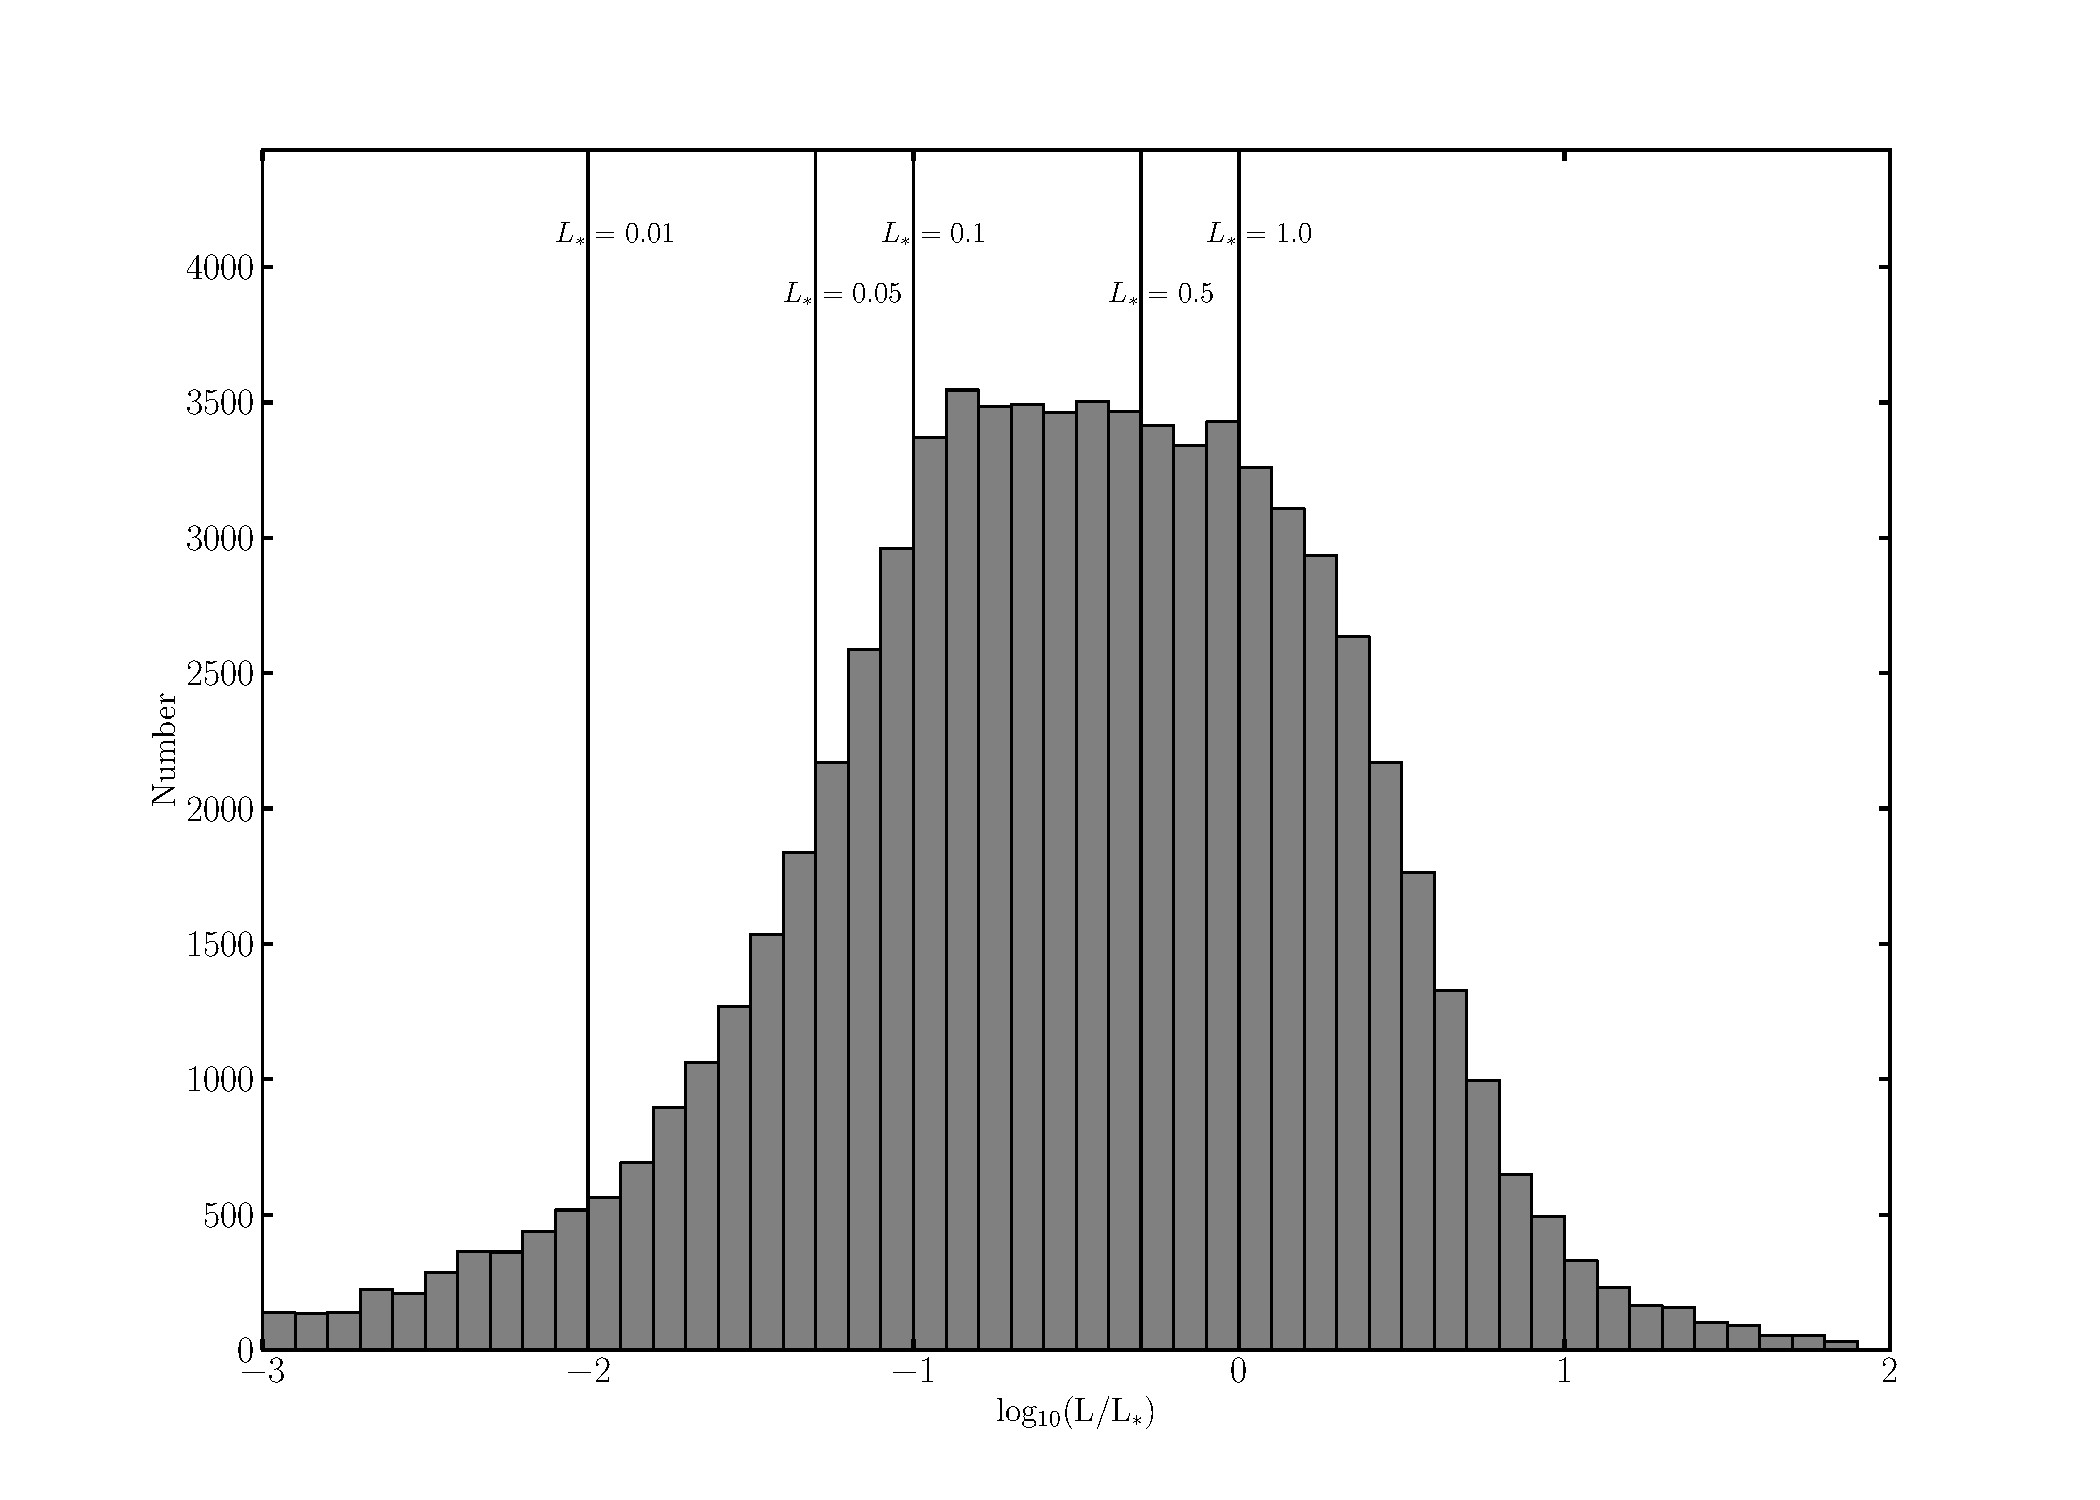
\includegraphics[width=0.52\textwidth]{completeness_hist.pdf}
        \caption{\small{Distribution of $L/L_{\**}$ values for all galaxies in the dataset. Black vertical lines highlight 1, 0.5, 0.1, 0.05 and 0.01 $L_{\**}$. The turnoff around 0.1$L_{\**}$ shows that on average, the dataset is complete to 0.1$L_{\**}$.}}
%        \vspace{-5pt}
        \label{completeness}
\end{figure} 

In addition, we have homogenized the galaxy data beyond the steps taken by NED by normalizing all measurements of galaxy inclination, position angle, and diameter to 2MASS $K$-band values. Most galaxies in NED have measures of inclination, position angle and diameter available in several different bands, so in order to make meaningful comparisons, it is necessary to choose one band for all measurements. We chose 2MASS values for this because it was an all-sky survey, and represents the largest fraction of available galaxy data. Physical galaxy diameters are derived from 2MASS $K_s$ ``total" angular diameter measurements and galaxy distances. 2MASS $K_s$ ``total" diameter estimates are surface brightness extrapolation measurements and are derived as 

\begin{equation}
r_{tot} = r' + a(ln(148)^b,
\end{equation}

\noindent where $r_{tot}$ is defined as the point where the surface brightness extends to 5 disk scale lengths, $r'$ is the starting point radius ($>5" - 10"$ beyond the nucleus, or core influence), and $a$ and $b$ are Sersic exponential function scale length parameters ($f = f_0 \exp{(-r/a)}^{(1/b)}$, see Jarret et al. 2003 for a full description). Approximately $50\%$ of all the galaxies have this 2MASS $K_s$ ``total" diameter. Of the remainder, $20\%$ have SDSS diameters, $27\%$ have no published diameter, and $3\%$ have diameters from other surveys. We convert values in these other bands to 2MASS $K_s$ ``total" diameters via a simple least squares linear fit when necessary. \textbf{NEEDS TO BE CHECKED FOR FULL SKY}

We used $B$-band magnitudes to estimate each galaxy's luminosity as a ratio of $L_{\**}$ as follows:

\begin{equation}
	\frac{L}{L_{\**}} = 10^{-0.4 (M_{B} - M_{B_{\**}})}.
\end{equation}

We adopt the CfA galaxy luminosity function by Marzke et al. (1994), which sets $B_{\**} $ = -19.57. Direct $B$ band measurements are available for $\sim 30\%$ of galaxies, and most of the rest have SDSS $g$ and $r$ magnitudes, which can be converted to $B$ via $B = g + 0.39 (g-r) + 0.21$ (Jester et al. 2005). Finally, we also compute an estimate of the virial radius of each galaxy as $log R_{vir} = 0.69 log D + 1.24$. This follows the parametrization of Stocke et al. (2013) relating a galaxy's luminosity to its virial radius, and the Wakker $\&$ Savage (2009) empirical relation between diameter and luminosity (see Wakker et al. 2015 and references therein for further details).

This homogeneous galaxy data table allows us to draw direct comparisons between the properties of the absorbers and the properties, separations, and environments of nearby galaxies, with unprecedented completeness. The full dataset will be publicly released and discussed in further detail in a forthcoming paper (French et al. 2016, in prep).


\begin{figure}[h!]
\centering
  \subfigure[]{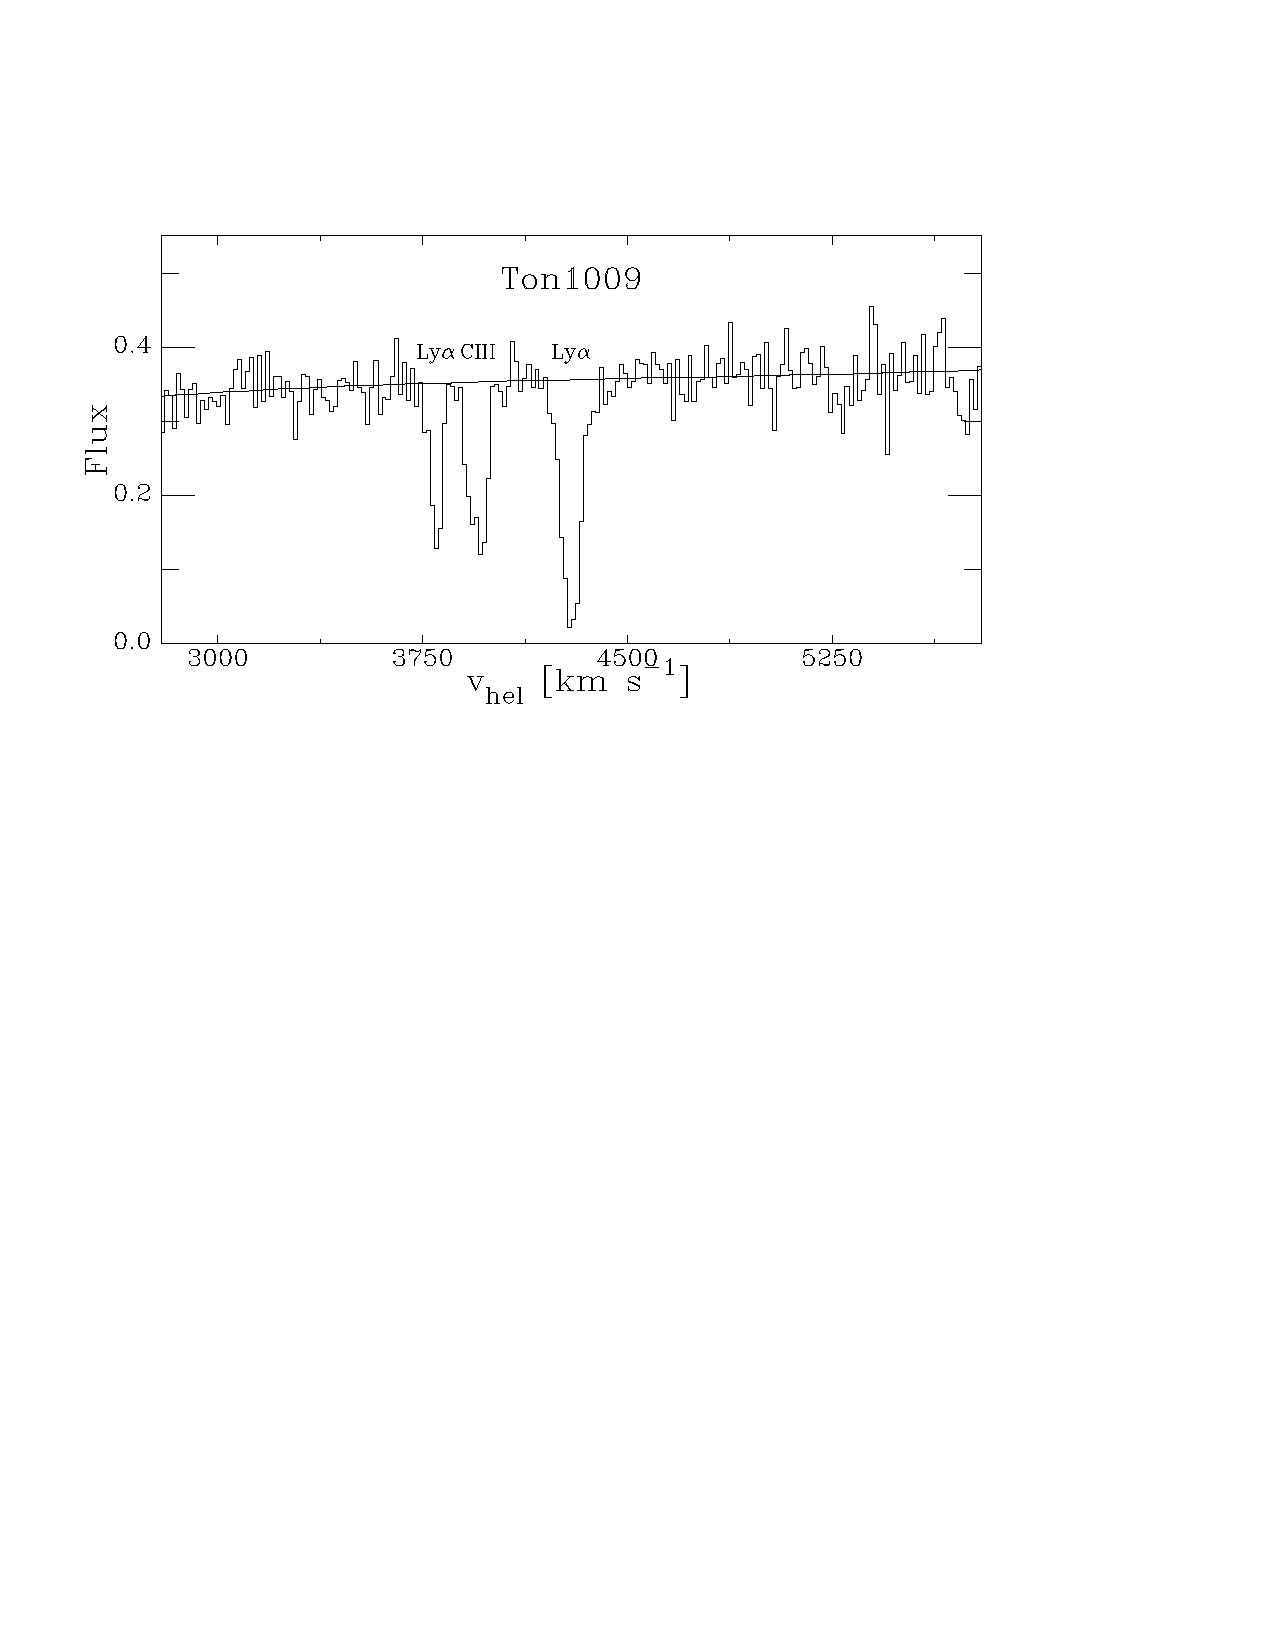
\includegraphics[width=1.\linewidth]{figTON1009_crop.pdf}}{\label{line}}
  \subfigure[]{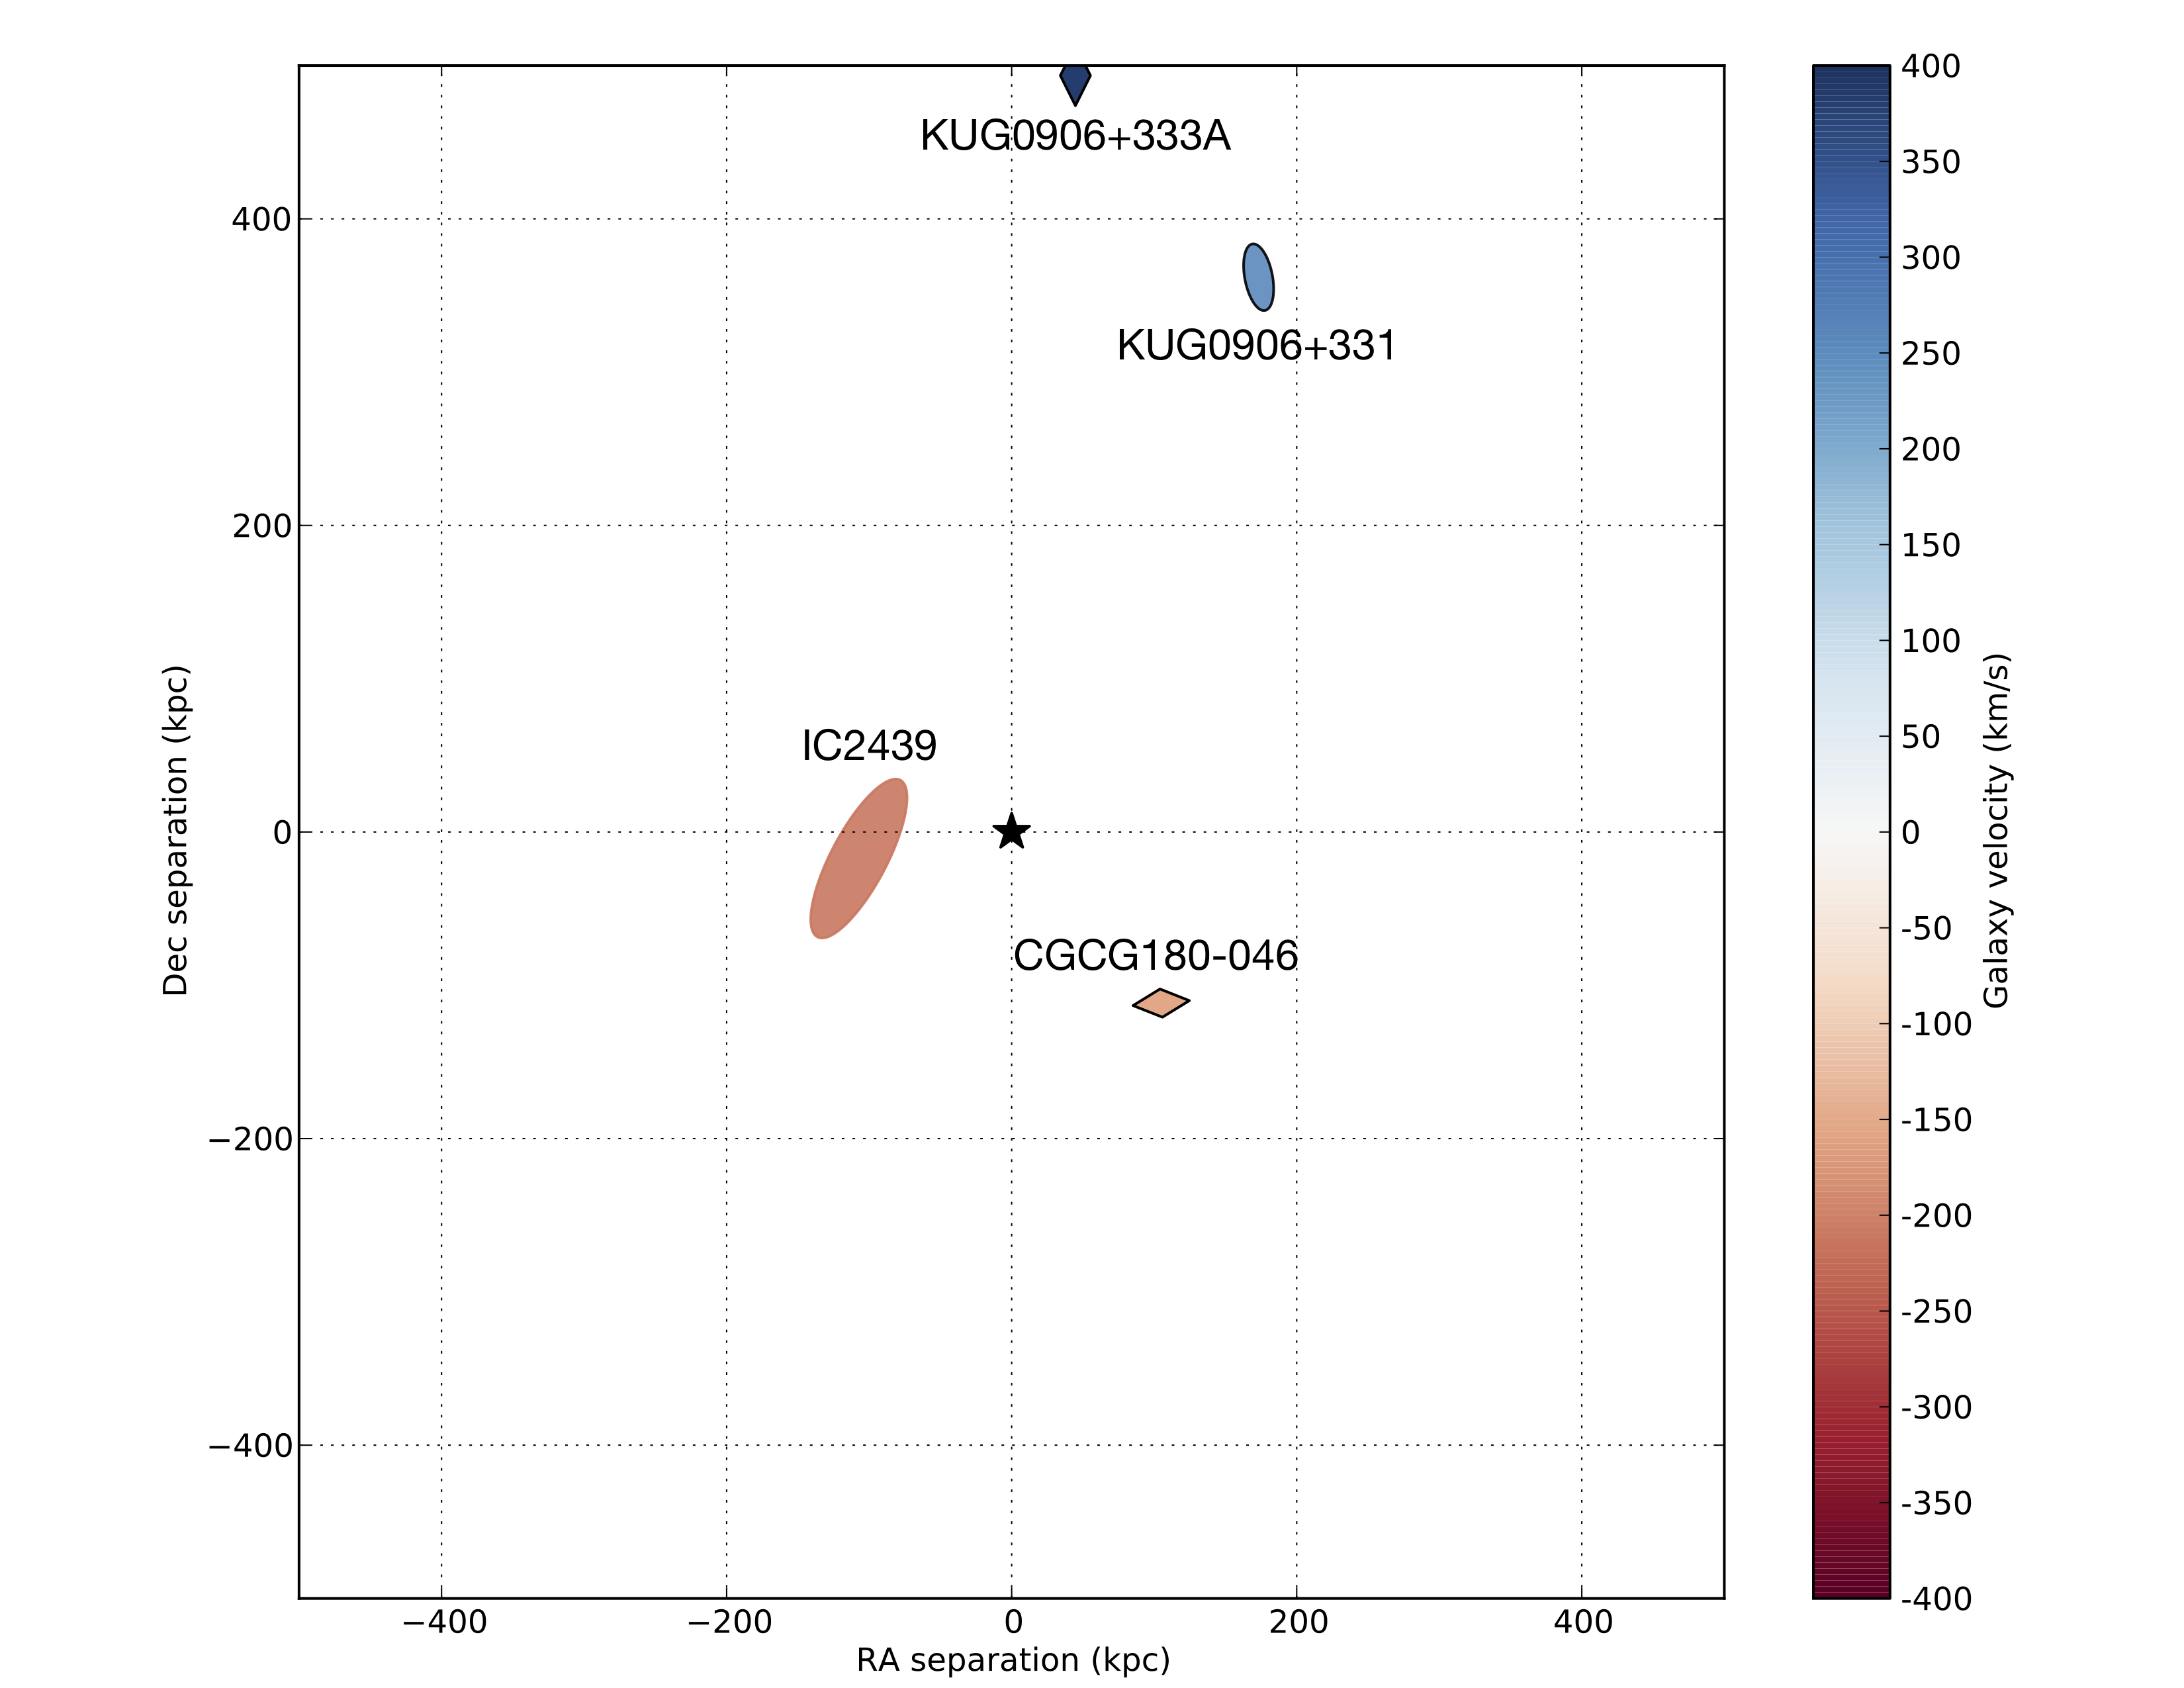
\includegraphics[width=1.\linewidth]{map_TON1009_4285_crop2_labels.png}\label{impactmap}}
  \caption{\small{a) An example Ly$\alpha$ line found in a sightline towards target TON1009 at 4295 km/s. b) A map of \textit{all} galaxies within a 500 kpc impact parameter target TON1009 sightline and with velocity ($cz$) within 400 km/s of absorption detected at 4295 km/s (central black star). The galaxy IC2439 ($v=4494$ km/s, inclination = $71^{\circ}$) can be unambiguously paired with the Ly$\alpha$ absorption feature at $v=4295$ km/s because it is the largest and closest galaxy in both physical and velocity space to the absorption feature.}}
\vspace{5pt}
\end{figure}


\subsection{Spectra}

This initial pilot study contains 35 sightlines to bright QSOs observed with COS (32 of 35) and STIS (3 of 35). We chose sightlines by first sorting the galaxy data table described above by diameter. This sorted list is then correlated with the full list of publicly available sightlines, and only systems with impact parameter less than 500 Mpc are kept. Finally, we reject any messy, overly complicated sightlines, or low S/N sightlines and select the top 35 (again, sorted by galaxy diameter). Table \ref{target_table} summarizes the properties of the QSO targets we selected.

%We chose sight lines based on high S/N (generally $>$10), ease of spectral identification, and proximity to large, nearby galaxies. Several are included simply because they already have published identifications. There were no strict cutoffs for galaxy size or brightness, we simply selected the top 35 sight lines after rejecting those with lower S/N and/or more complicated features. 

All COS spectra for the target sightlines were obtained through the Barbara A. Mikulski Archive for Space Telescopes (MAST), and processed with CALCOS v3.0. We combined individual exposures by the method of Wakker et al. (2015), which corrects the COS wavelength scale by cross-correlating all ISM and IGM lines in each exposure. This method addresses the up to $\pm40$ km/s misalignments produced by CALCOS, and produces a corrected error array based on Poisson noise, which better matches the measured errors then the errors delivered in the x1d files. We then combine multiple exposure by aligning Galactic absorption lines with 21-cm spectra, and adding up the total counts in each pixel before converting to flux using the original, average flux-count ratio at each wavelength.

For STIS observations, the calibrated fits files were downloaded from MAST, and STIS-E140M echelle orders were combined into a single spectrum. The photon counts and errors were interpolated onto a common grid, 

Spectra taken with the STIS-E140M echelle were ..... \textbf{FINISH THIS - SEE W\&S 2009}


\begin{table*}[ht]\footnotesize
\begin{center}
\begin{tabular}{l l l c c c c c c c c c c c c}
 \hline \hline
  Target & Galaxy & $\mathcal{L}$ & $R_{vir}$ & $\rho$ (kpc) & $v_{galaxy}$ & $\Delta v$  &  Inc.   &  Az.     & $v_{Ly\alpha}$ & $$W$_{Ly\alpha}$ \\ 
  	     &               &                      & \scriptsize [kpc] & \scriptsize [kpc] & \scriptsize [km/s] & \scriptsize [km/s] & \scriptsize [deg] & \scriptsize [deg] & \scriptsize [km/s] & \scriptsize [m\AA]	\\
 \scriptsize (1) & \scriptsize (2) & \scriptsize (3) & \scriptsize (4) & \scriptsize (5) & \scriptsize (6) & \scriptsize  (7) & \scriptsize (8) & \scriptsize (9) & \scriptsize (10) & \scriptsize (11) \\ \hline \hline
SBS1537+577 & SDSSJ153802.75+573018.3 & 0.0076 & 87 & 91 & 3687 & -389.7 & 80 & 15 & 4077 & 72$\pm$25\\
SDSSJ080838.80+051440.0 & 2MASXJ08083956+0517256 & 0.0083 & 106 & 106 & 9371 & -389 & 26 & 71 & 9760 & 58$\pm$15\\
MRK1014 & NGC0768 & 0.0087* & 253 & 486 & 6752 & -327.7 & 73 & 85 & 7080 & 117$\pm$11\\
MRC2251-178 & MCG-03-58-009 & 0.16* & 319 & 320 & 8754 & -297.2 & 59 & 39 & 9051 & 60$\pm$4\\
RX\_J1503.2+6810 & CGCG318-012 & 0.25* & 250 & 325 & 9912 & -210.2 & 50 & 1 & 10122 & 44$\pm$14\\
2dFGRS\_S393Z082 & NGC1097 & 0.62* & 273 & 112 & 1030 & -209.2 & 47 & 12 & 1239 & 570$\pm$21\\
HE1228+0131 & NGC4517 & 0.19 & 193 & 211 & 1420 & -135.6 & 83 & 74 & 1556 & 20$\pm$2\\
SBS1537+577 & NGC5987 & 0.79* & 322 & 454 & 3170 & -109 & 65 & 33 & 3279 & 358$\pm$30\\
HE1228+0131 & NGC4517 & 0.27 & 193 & 211 & 1420 & -67.6 & 83 & 74 & 1488 & 144$\pm$3\\
PG1302-102 & NGC4939 & 0.77* & 235 & 265 & 3382 & -66.2 & 46 & 61 & 3448 & 71$\pm$5\\
MRC2251-178 & HIPASSJ2254-18 & 0.00096 & 122 & 320 & 2991 & -51.5 & 53 & 56 & 3042 & 67$\pm$5\\
PG0003+158 & NGC7814 & 0.25 & 171 & 197 & 789 & -43.7 & 65 & 47 & 833 & 131$\pm$15\\
MRK290 & NGC5987 & 0.94* & 322 & 486 & 3170 & -37 & 65 & 12 & 3207 & 319$\pm$4\\
SDSSJ080838.80+051440.0 & UGC04239 & 0.85* & 279 & 378 & 8893 & -33.9 & 44 & 38 & 8927 & 130$\pm$19\\
SBS1108+560 & UGC06225 & 2.0 & 228 & 29 & 910 & -18.6 & 77 & 82 & 929 & 284$\pm$51\\
RX\_J0714.5+7408 & UGC03717 & 0.18* & 202 & 271 & 4269 & 4.8 & 61 & 83 & 4264 & 410$\pm$9\\
1H0717+714 & UGC03804 & 0.24 & 173 & 207 & 2973 & 16.8 & 53 & 7 & 2956 & 39$\pm$4\\
MRK290 & NGC5987 & 0.87* & 322 & 486 & 3170 & 65 & 65 & 12 & 3105 & 511$\pm$5\\
1H0717+714 & UGC03804 & 0.18 & 173 & 207 & 2973 & 102.8 & 53 & 7 & 2870 & 343$\pm$6\\
SDSSJ080908.13+461925.6 & SDSSJ080842.74+461828.9 & 0.14 & 103 & 133 & 7227 & 110.2 & 37 & 4 & 7117 & 176$\pm$12\\
PG1307+085 & CGCG072-007 & 0.0036 & 193 & 440 & 7413 & 134.2 & 50 & 43 & 7279 & 64$\pm$7\\
SBS1537+577 & SDSSJ153802.75+573018.3 & 0.21 & 87 & 91 & 3687 & 138.3 & 80 & 15 & 3549 & 447$\pm$28\\
SDSSJ080838.80+051440.0 & UGC04239 & 0.49* & 279 & 378 & 8893 & 153.1 & 44 & 38 & 8740 & 883$\pm$24\\
SBS1108+560 & UGC06225 & 0.89 & 228 & 29 & 910 & 178.4 & 77 & 82 & 732 & 1082$\pm$82\\
TON1009 & NGC2770 & 0.083* & 204 & 274 & 2143 & 182.1 & 78 & 43 & 1961 & 350$\pm$21\\
3C273.0 & SDSSJ122815.96+014944.1 & 0.0034 & 41 & 91 & 1198 & 185.4 & 59 & 3 & 1013 & 376$\pm$3\\
SBS1122+594 & IC0691 & 0.53 & 66 & 45 & 1399 & 185.4 & 42 & 56 & 1214 & 830$\pm$13\\
RX\_J0714.5+7408 & UGC03717 & 0.069* & 202 & 271 & 4269 & 194.8 & 61 & 83 & 4074 & 58$\pm$7\\
TON1009 & IC2439 & 0.4 & 153 & 109 & 4495 & 209.8 & 71 & 51 & 4285 & 343$\pm$17\\
TON488 & UGC05478 & 0.3 & 92 & 58 & 1620 & 245.3 & 12 & x & 1375 & 452$\pm$12\\
RX\_J1330.8+3119 & UGC08496NED02 & 0.014 & 101 & 160 & 5104 & 265.2 & 59 & 46 & 4839 & 413$\pm$16\\
H1101-232 & MCG-04-26-019 & 0.058 & 173 & 179 & 3846 & 266.2 & 65 & 26 & 3580 & 573$\pm$12\\
RX\_J1330.8+3119 & UGC08492 & 0.01* & 204 & 335 & 7689 & 288.2 & 16 & 41 & 7401 & 330$\pm$15\\
SDSSJ140428.30+335342.0 & KUG1402+341 & 0.17 & 204 & 118 & 8178 & 293.5 & 69 & 63 & 7884 & 889$\pm$28\\
PG1211+143 & NGC4189 & 0.0053 & 181 & 314 & 2415 & 298.5 & 55 & 84 & 2116 & 105$\pm$8\\
CSO395 & UGC07207 & 0.11 & 103 & 83 & 1324 & 299.4 & 61 & x & 1025 & 343$\pm$15\\
PG1121+423 & SDSSJ112418.74+420323.1 & 0.023 & 104 & 129 & 7628 & 300 & 65 & 20 & 7328 & 359$\pm$7\\
PG1216+069 & SDSSJ121903.72+063342.9 & 0.0072 & 71 & 110 & 4131 & 318 & 61 & 65 & 3813 & 360$\pm$10\\
SDSSJ080908.13+461925.6 & SDSSJ080842.74+461828.9 & 0.013 & 103 & 133 & 7227 & 327.2 & 37 & 4 & 6900 & 151$\pm$10\\
PG1121+423 & SDSSJ112418.74+420323.1 & 0.01 & 104 & 129 & 7628 & 349 & 65 & 20 & 7279 & 46$\pm$6\\
TON488 & UGC05478 & 0.044 & 92 & 58 & 1620 & 370.3 & 12 & x & 1250 & 68$\pm$9\\
HE1228+0131 & 2MASXJ12303439+0116243 & 0.0063 & 127 & 159 & 9613 & 373.8 & 28 & 60 & 9239 & 249$\pm$3\\
 \\
\hline
\end{tabular}
\end{center}
  \caption{\small{All associated systems. The largest $\mathcal{L}$ value is given, where a (\**) indicates $d^{1.5}$ was used, otherwise the quoted $\mathcal{L}$ was computed with $R_{vir}$. For all entries, 'x' indicates unknown values.}}
  \label{target_table}
\end{table*}


\begin{figure}[ht!]
  \centering
  \subfigure[]{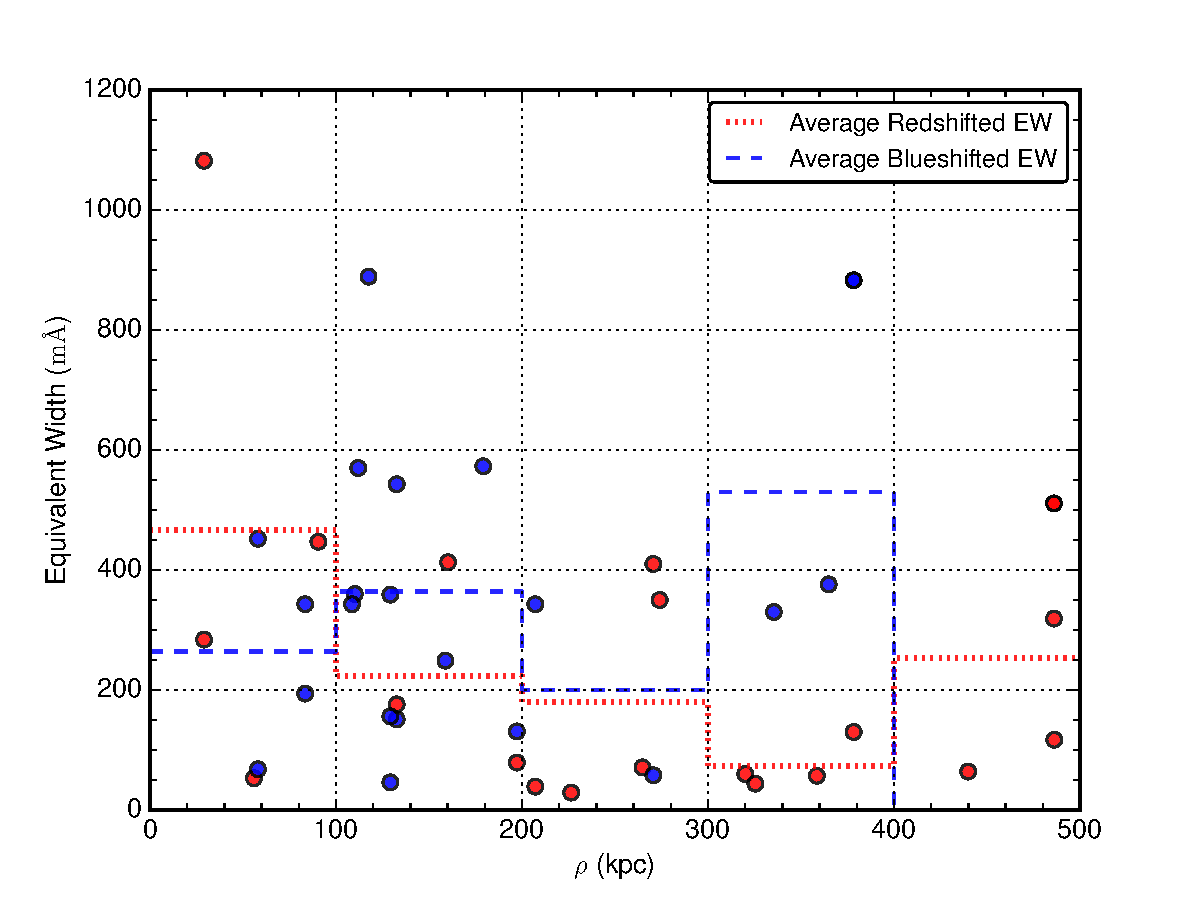
\includegraphics[scale=0.46]{W(impact)_avgHistograms.pdf}}{\label{ew_vs_impact}}
  \subfigure[]{\includegraphics[scale=0.46]{W(impact_vir)_avgHistograms.pdf}}{\label{ew_vs_impact-d}}
  \caption{a) Equivalent width ($W$) of each absorber as a function of $\rho$ (kpc), the physical impact parameter between the galaxy and the sightline toward the absorption feature. b) ($W$) as a function of $\rho/R_{vir}$, the ratio of the physical impact parameter and the galaxy diameter. The anti-correlation is strongest when scaling $\rho$ by the galaxy virial radius.}
 \label{ew_both}
\end{figure}
\vspace{10pt}


\section{Results}

We have identified 175 Ly$\alpha$ absorption lines in the spectra of 35 background QSOs. Of these, $24\%$ can be unambiguously associated with a single nearby galaxy, while $53\%$ reside greater than $\rho = 500$ kpc and $\Delta v = 400$ km/s from any galaxy. In order to be considered for a pairing, a galaxy and absorption feature must appear within 400 km/s in velocity and 500 kpc in physical impact parameter from each other. When multiple galaxies pass these criteria for a particular line, we are left with two options. 1) one galaxy is obviously far larger and closer in physical and velocity space to the line, and may have several satellite galaxies, or 2) no single galaxy if obviously dominant, and we do not include this line in further analysis. 

To facilitate this decision, we compute the likelihood, $\mathcal{L}$, of every possible galaxy-absorber pairing as follows:

\begin{equation}
	\mathcal{L} = A e^{-(\frac{\rho}{R})^2} e^{-(\frac{\Delta v}{200})^2}.
\end{equation}

\noindent Here $\rho$ is the physical impact parameter, $\Delta v$ the velocity difference between the absorber and the galaxy ($\Delta v = v_{galaxy} - v_{absorber}$), and $A$ is a factor included to increase the likelihood in the case that $R \geq \rho$ (in which case $A = 2$, otherwise $A = 1$). We compute $\mathcal{L}$ for two different values of $R$: $R_{vir}$, the virial radius of the galaxy, and $d^{1.5}$, the major diameter of the galaxy to the power of 1.5. $\mathcal{L}$ computed with $R_{vir}$ is liable to select satellite galaxies instead of the larger hosts, so including a version with $d^{1.5}$ serves as a two-tiered selection system. An absorber-galaxy system separated by 200 km/s in velocity and 1$R_{vir}$ would have $\mathcal{L} = 0.27$. In order for an absorber to be marked as ``associated" with a particular galaxy, its $\mathcal{L}$ must be a factor of 5 larger than the next best possible association, and $\mathcal{L} \ge 0.001$. We then visually inspect each system before it is included in the final sample, rejecting associations with galaxies residing in complex or group environments.

\begin{figure}[h!]
        \centering
        \includegraphics[width=0.52\textwidth]{W(vir)_avgHistograms.pdf}
        \caption{\small{Equivalent width ($W$) of each absorber as a function of the virial radius of the associated galaxy in the sample. The blue-dotted and red-dashed lines shows the average $W$ in 50 kpc bins of $R_{vir}$ for the blueshifted and redshifted absorbers, respectively.}}
        \label{w_vir}
        \vspace{2pt}
\end{figure} 


Figures \ref{line} and \ref{impactmap} show a clean example of a Ly$\alpha$ absorption line with a map of its galaxy environment, showing an unambiguous pairing between the absorption feature at $4295$ km/s toward TON1009 and galaxy IC2439 ($\mathcal{L} = 0.45$). Unless explicitly stated, all following analysis concerns similarly unambiguous ``associated" systems.


Most interestingly, new results emerge when we split the absorber-galaxy catalog based on the velocity difference of the two. We define the differential velocity between the absorption feature and an associated galaxy as follows:

\begin{equation}
	\Delta v = v_{galaxy} - v_{absorber}.
\end{equation}

With this scheme, we refer to an absorber with a velocity \textit{lower} than the associated galaxy as \textit{blueshifted}, while an absorber with a velocity \textit{higher} is referred to as \textit{redshifted}. The rest of the results will be analyzed based upon this splitting. For all distributions, we employ and quote the results of both the Kolmogorov-Smirnov (KS) and the Anderson-Darling (AD) statistical tests.

%\begin{figure}[h!]
%\centering
%  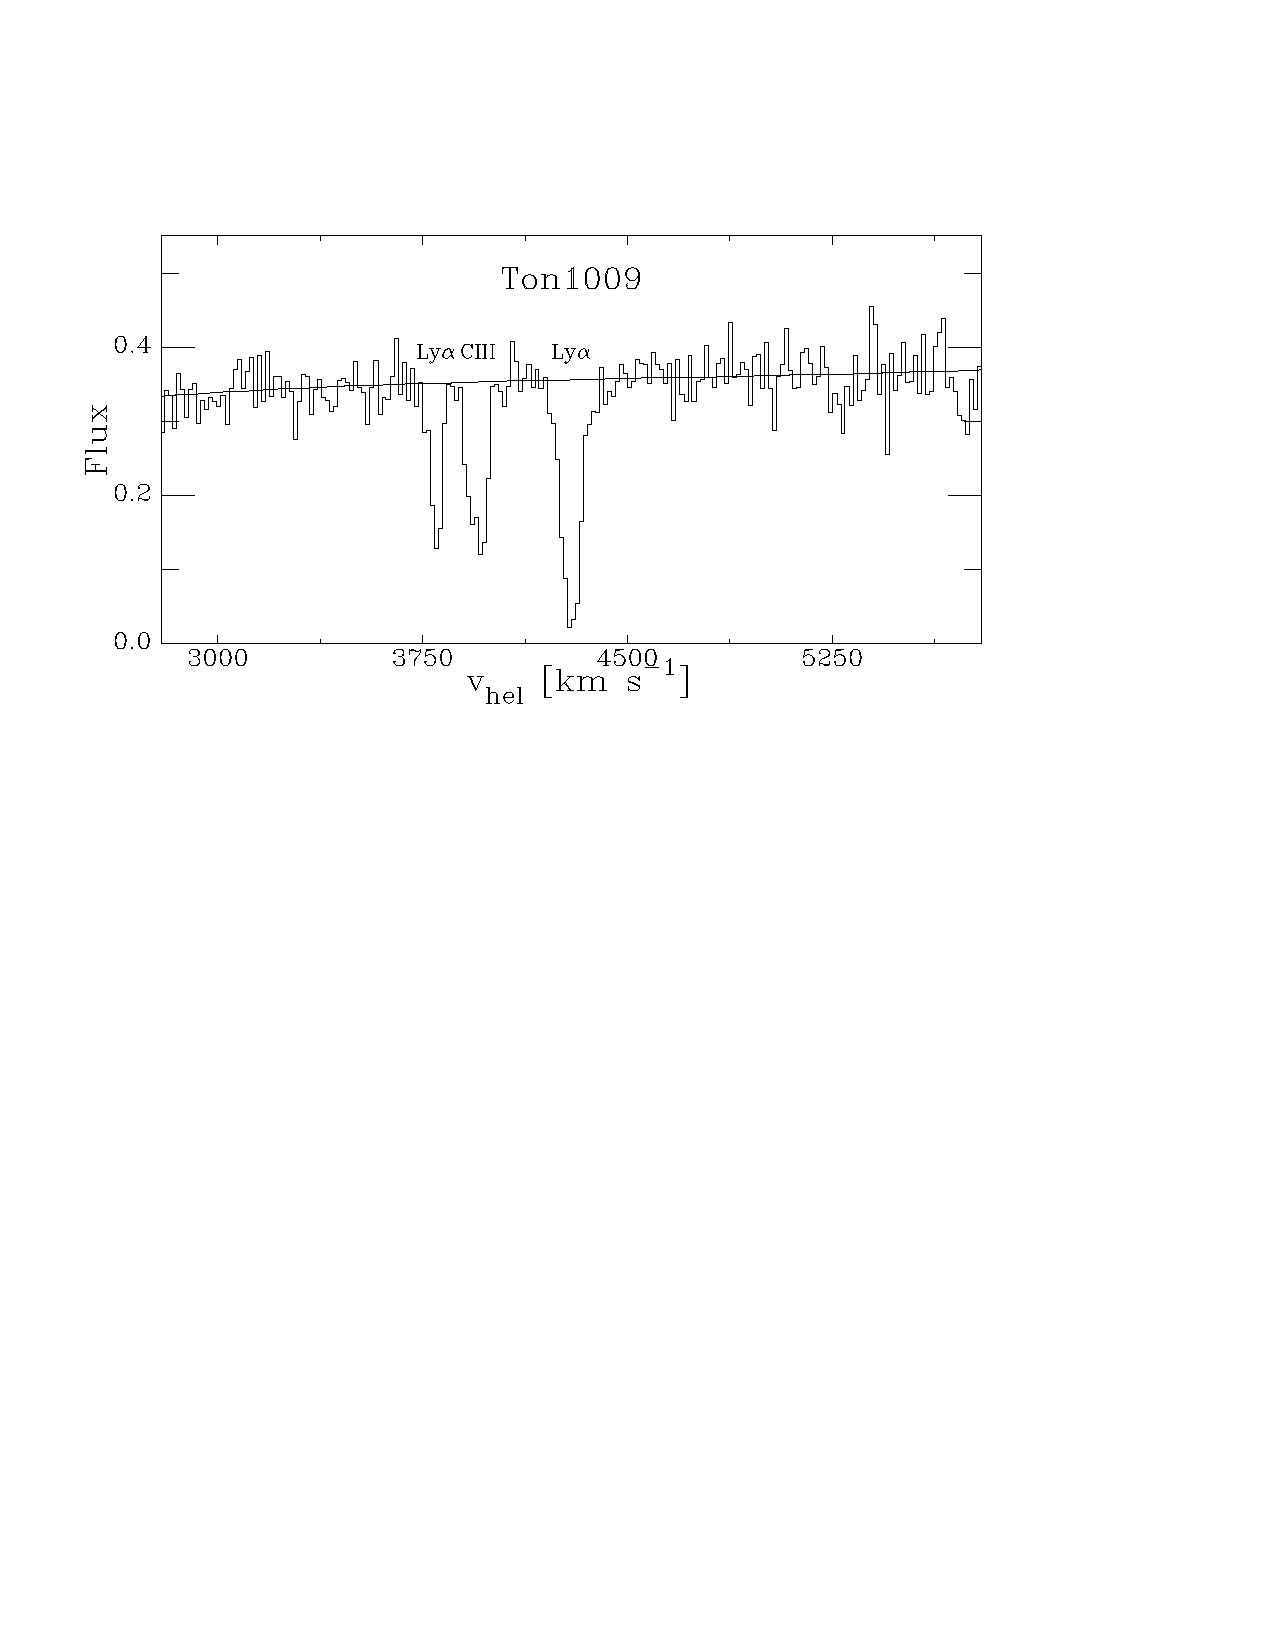
\includegraphics[width=1.\linewidth]{figTON1009_crop.pdf}
%  \caption{\small{An example Ly$\alpha$ line found in a sightline towards target TON1009 at 4295 km/s.}}
%  \label{line}
%\end{figure}
%\begin{figure}[h!]
%  \centering
%  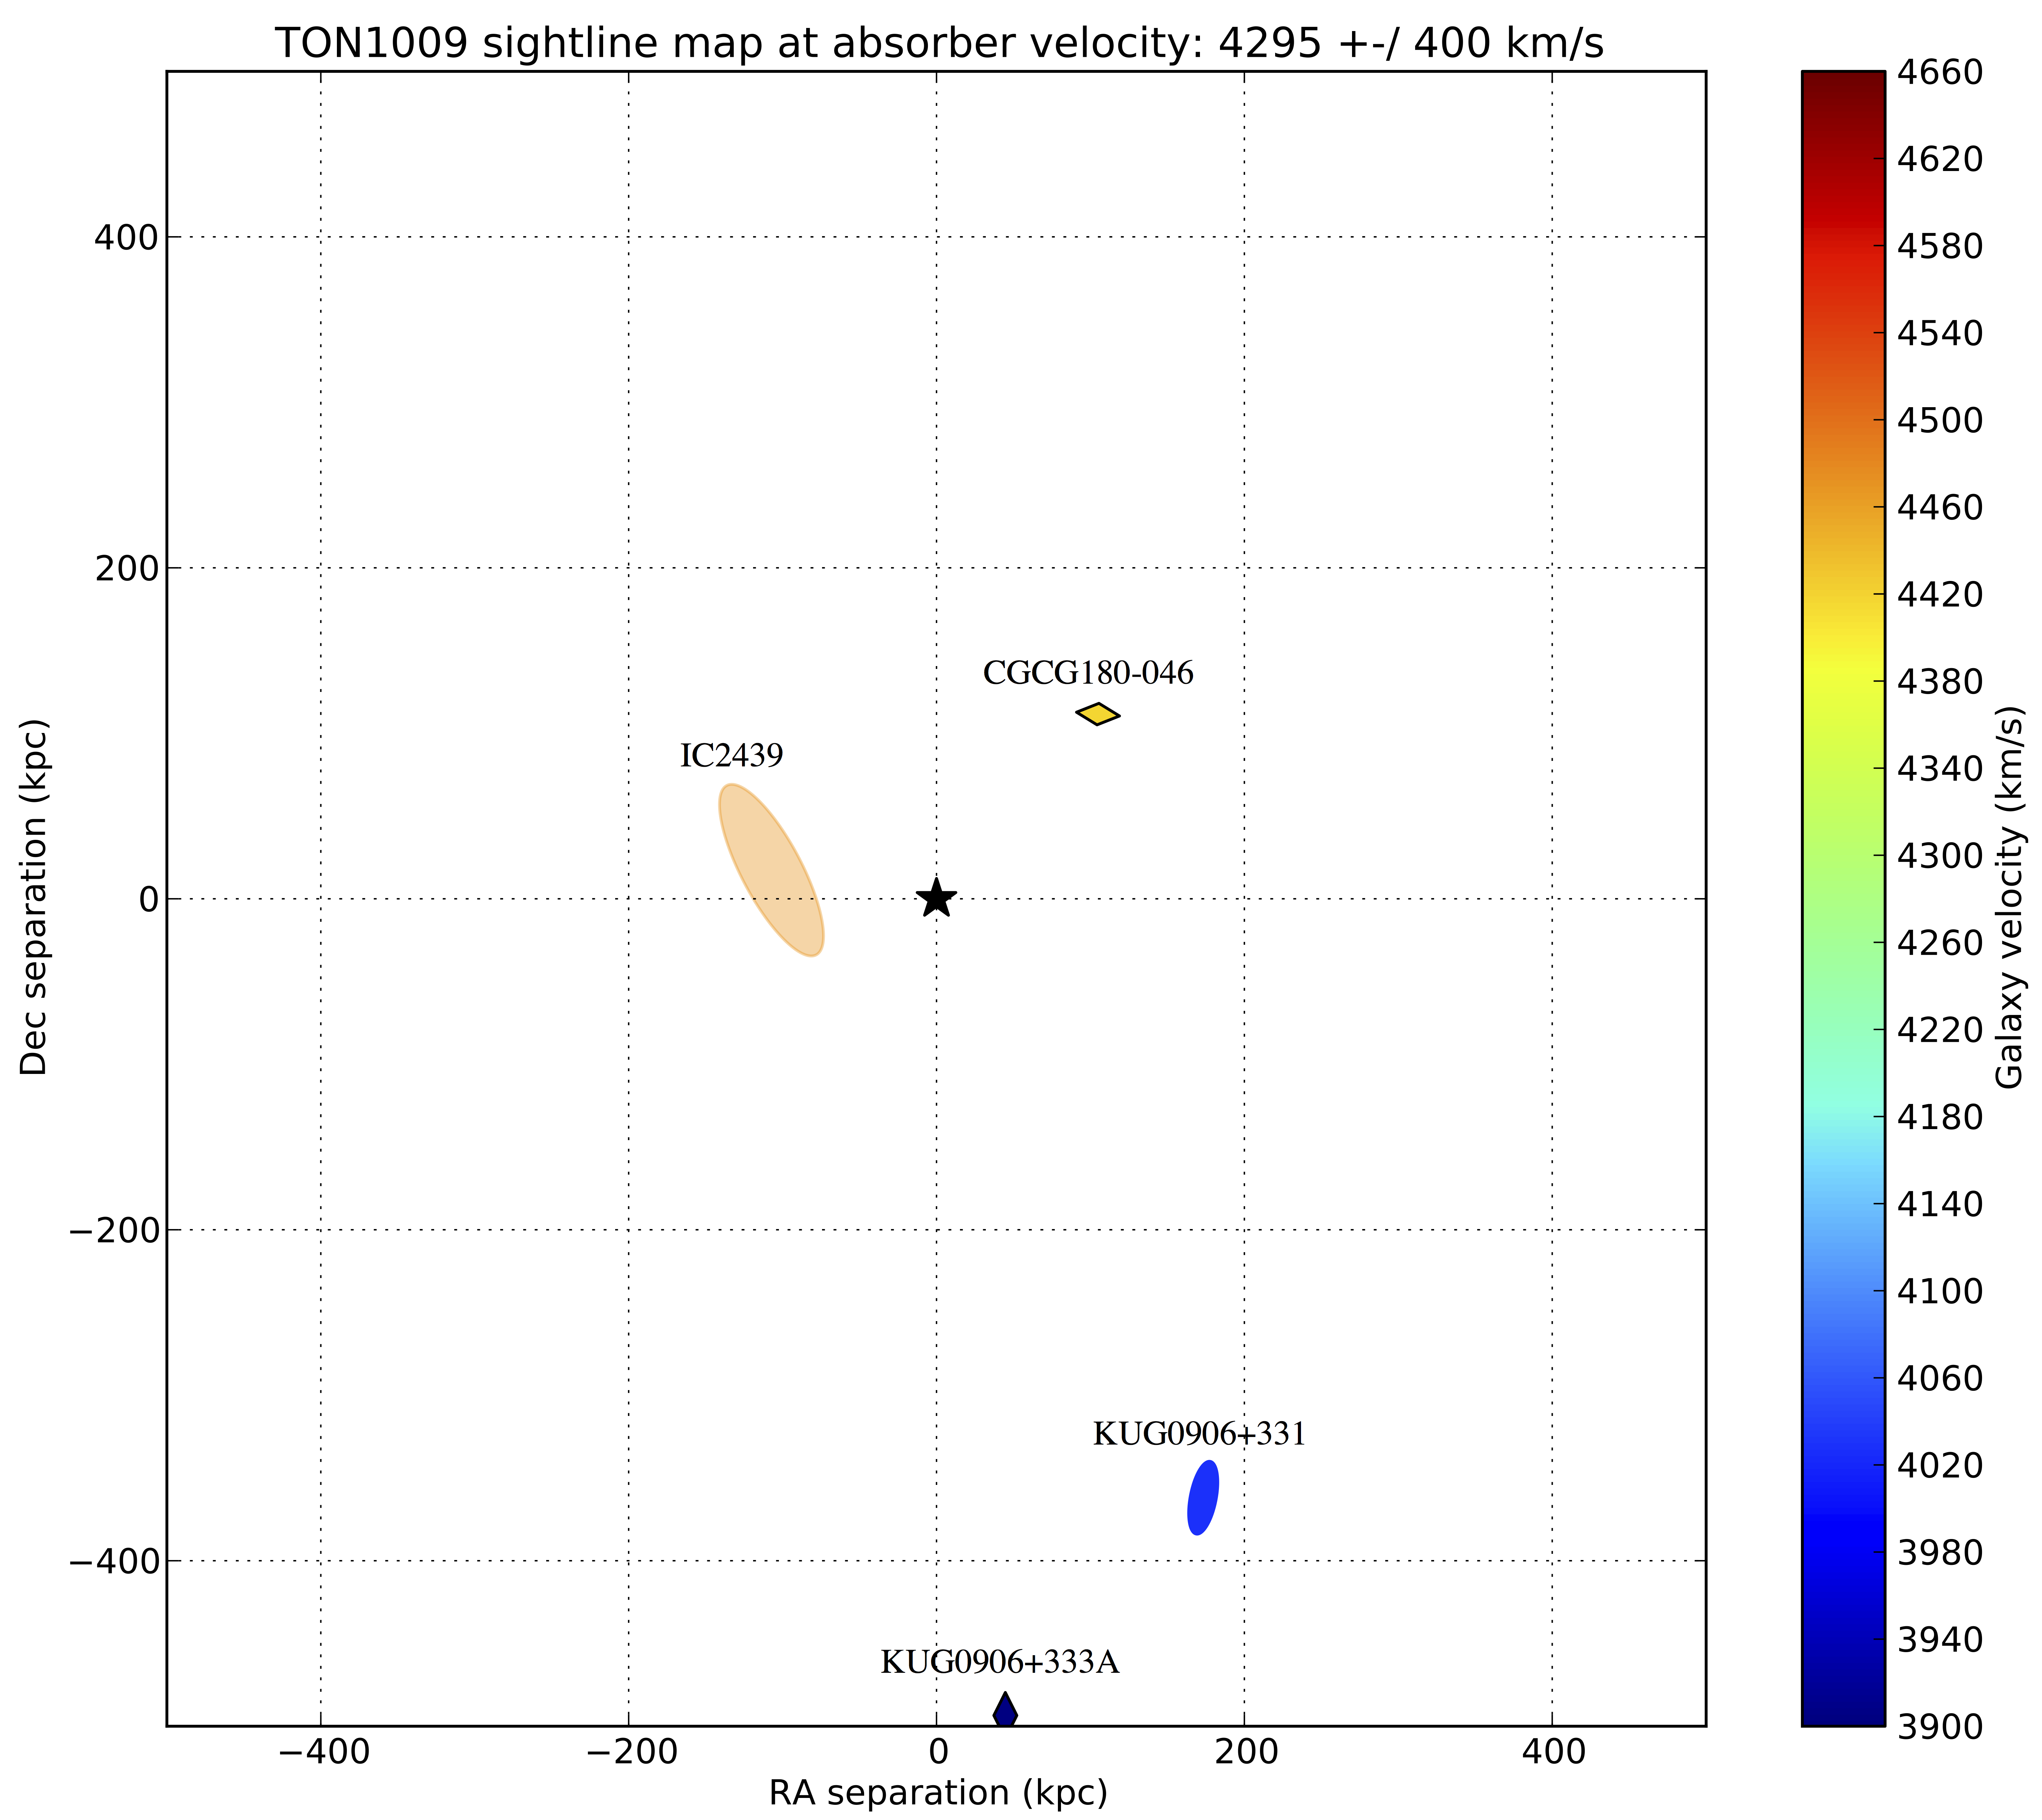
\includegraphics[width=1.\linewidth]{map2_TON1009_4295_newlabels_crop_hires2.png}
%  \caption{\small{A map of \textit{all} galaxies within a 500 kpc impact parameter target TON1009 sightline and with velocity ($cz$) within 400 km/s of absorption detected at 4295 km/s (central black star). The galaxy IC2439 ($v=4494$ km/s, inclination = $71^{\circ}$) can be unambiguously paired with the Ly$\alpha$ absorption feature at $v=4295$ km/s because it is the largest and closest galaxy in both physical and velocity space to the absorption feature.}}
%  \label{impactmap}
%\label{TON1009}
%\vspace{5pt}
%\end{figure}


\subsection{W-$\rho$ Anti-correlation}
As mentioned earlier, numerous previous studies have found that Ly$\alpha$ equivalent width ($W$) is anti-correlated with impact parameter ($\rho$) to the nearest galaxy. We find a weak correlation, as shown in Figure \ref{ew_both}(a). However, we find a stronger anti-correlation when we normalize $\rho$ by $R_{vir}$. Figure \ref{ew_both}(b) shows this expected anti-correlation when plotting $W$ vs $\rho/R_{vir}$. The obvious explanation for this is that larger galaxies host larger, more physically extent CGM halos. We would thus expect $W$ to also correlate positively with $R_{vir}$. Figure \ref{w_vir} shows $W$ as a function of $R_{vir}$, with the blue-dotted and red-dashed lines show the average $W$ in bins of 50 kpc of $R_{vir}$. A slight, positive correlation is evident between equivalent width and galaxy virial radius.


%\begin{figure*}[h!]
%\centering
%\begin{minipage}[b]{.49\textwidth}
%        \includegraphics[width=0.52\textwidth]{W(impact)_dif.pdf}
%        \caption{\small{Equivalent width ($W$) of each absorber as a function of $\rho$ (kpc), the physical impact parameter between the galaxy and the sightline toward the absorption feature. Only a slight anti-correlation can be seen.}}
%        \label{ew_vs_impact}
%\end{minipage}\hfill
%\begin{minipage}[b]{.49\textwidth}
%        \includegraphics[width=0.52\textwidth]{W(impact_diam)_dif.pdf}
%        \caption{\small{Equivalent width ($W$) of each absorber as a function of $\rho$/D, the ratio of the physical impact parameter and the galaxy diameter. A strong anti-correlation is evident.}}
%%        \vspace{-5pt}
%        \label{ew_vs_impact-d}
%\end{minipage}
%\end{figure*}


%\begin{figure}[h!]
%        \centering
%        \vspace{-10pt}
%        \includegraphics[width=0.52\textwidth]{W(impact)_dif.pdf}
%        \caption{\small{Equivalent width ($W$) of each absorber as a function of $\rho$ (kpc), the physical impact parameter between the galaxy and the sightline toward the absorption feature. Only a slight anti-correlation can be seen.}}
%%        \vspace{-5pt}
%        \label{ew_vs_impact}
%\end{figure} 
%
%\begin{figure}[h!]
%        \centering
%        \vspace{-10pt}
%        \includegraphics[width=0.52\textwidth]{W(impact_diam)_dif.pdf}
%        \caption{\small{Equivalent width ($W$) of each absorber as a function of $\rho$/D, the ratio of the physical impact parameter and the galaxy diameter. A strong anti-correlation is evident.}}
%%        \vspace{-5pt}
%        \label{ew_vs_impact-d}
%\end{figure} 


\begin{figure}[h!]
        \centering
        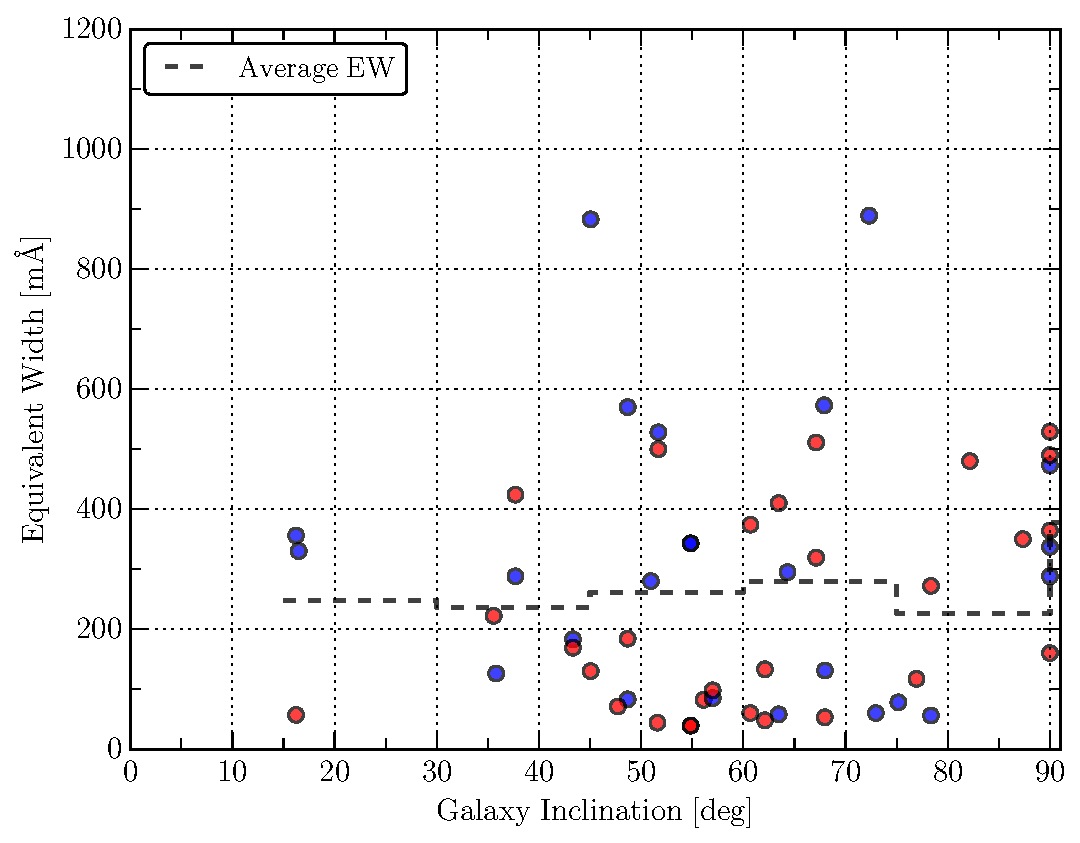
\includegraphics[width=0.52\textwidth]{W(inc)_medHistogram.pdf}
        \caption{\small{Equivalent width ($W$) of each absorber as a function of the inclination angle of the associated galaxy in the pilot study sample. The dashed black line is drawn to highlight the separation between red and blue shifted absorption systems (with respect to the systemic velocity of the galaxy).}}
        \label{ew_vs_inclination}
        \vspace{2pt}
\end{figure}

\begin{figure}[h!]
        \centering
        \includegraphics[width=0.52\textwidth]{hist(fancy_inclination)_red_blue_full_all.pdf}
        \caption{\small{\textbf{Top: }Distribution of inclinations for all associated galaxies, split into red and blue shifted sets on. \textbf{Bottom:} Distribution of inclination angles for all galaxies in the $cz \leq 10,000$ km/s redshift range.}}
        \label{ew_vs_inclination}
        \vspace{2pt}
\end{figure}



% for steeper line:
 % y = 6.33*inc + -100
% 
% for shallower line:
% y = 3.88*inc + -25
  
%\subsection{Virial Radius}
%
%We find a positive correlation between the impact parameter, and the virial radius of the associated galaxy. Figure \ref{impact_virial} illustrates this. Blue and red-shifted absorbers are found at all impact parameters, but redshifted absorbers appear to be found more commonly around larger galaxies. The mean $R_{vir}$ for a galaxy associated with a blueshifted absorber is 153 kpc, compared to 235 kpc for redshifted absorbers (significant at a $>98\%$ confidence level).
%
%\begin{figure}[h!]
%        \centering
%        \includegraphics[width=0.52\textwidth]{impact(virial).pdf}
%        \caption{\small{The impact parameter between the absorber and associated galaxy is plotted as a function of the virial radius of the galaxy.}}
%        \label{impact_virial}
%        \vspace{2pt}
%\end{figure} 


\subsection{Inclination}
In this section we examine the inclinations of the associated galaxies compared to the red and blueshifted distributions of absorbers. We compute galaxy inclination, $i$, as follows:

\begin{equation}
	\cos(i) = \sqrt{\frac{q^2 - q_0^2}{1 - q_0^2}},
\end{equation}

\noindent where $q = b/a$, the ratio of the minor to major axis, and $q_0$ is the intrinsic axis ratio, set to $q_0 = 0.2$ for all galaxies.

Figure \ref{ew_vs_inclination} shows red and blueshifted absorbers' $W$ plotted against the inclinations of their associated galaxies. We note that there is a clear dichotomy between the distributions, where blue shifted absorbers appear around nearly all inclinations of galaxies, but redshifted absorbers appear preferentially near highly-inclined galaxies ($i \geq$ 50 deg). In addition, redshifted absorbers appear with lower $W$ than those blueshifted across all inclinations. The average $W$ of all redshifted absorbers is $\langle W \rangle$ = $163 \pm 15$  $\textrm{m\AA}$, compared to $\langle W \rangle$ = $380 \pm 14$ $\textrm{m\AA}$ for blueshifted absorbers. We can reject the null hypothesis that red and blue shifted absorbers come from the same underlying distribution at the $99\%$ level (results of both KS and AD tests). 

In total, $70\%$ of blueshifted and $73\%$ of redshifted absorbers are associated with high inclined galaxies ($i \geq$ 50 deg). $56\%$ of all galaxies in the survey volume are highly inclined, indicating a slight preference for detecting absorption around inclined galaxies. However, KS and AD tests do not assign high significance to this result (p-values $\sim0.06$).

\begin{figure}[h!]
        \centering
        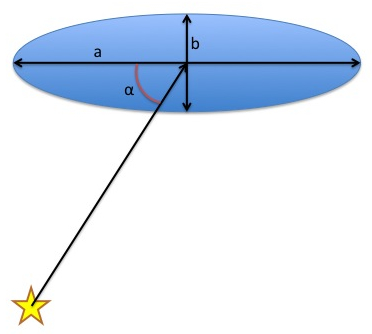
\includegraphics[width=0.35\textwidth]{azimuth_illustration_cut.jpg}
        \caption{\small{Azimuth is the angle, $\alpha$, between the major axis of the galaxy, $a$, and a vector extending from the AGN target to the galaxy center.}}
        \label{azimuth_illustration}
\end{figure} 

\begin{figure}[h!]
        \centering
        \includegraphics[width=0.51\textwidth]{hist(azimuth)_dif_10.pdf}
        \caption{\small{The distributions of azimuth angles for redshifted systems (top, red), and blueshifted systems (bottom, blue).}}
        \label{azimuth_dist}
        \vspace{5pt}
\end{figure} 

\subsection{Azimuth}
In this section we examine properties of absorbers as a function of their azimuthal angle with respect to their associated galaxy. Azimuth is defined as the angle between the major axis of a galaxy and the vector connecting the absorption feature and the midpoint of the galaxy plane. Figure \ref{azimuth_illustration} illustrates this. The mean azimuth angle for blueshifted absorbers is $40^{\circ}$, and $47^{\circ}$ for redshifted absorbers. Figure \ref{azimuth_dist} shows the distribution of azimuth angles for both red and blue-shifted absorbers. Contrary to the findings of Kacprzak et al. (2011, 2012), who claim to find a bimodal distribution of Mg\,{\sc ii} absorbers around galaxies, our distributions of Ly$\alpha$ absorbers are consistent with a flat, random distribution. There is a slight overabundance of absorbers around $0^{\circ}$ and $45^{\circ}$ azimuth in the blueshifted sample, but we cannot assign this observation much significance given the small sample size. We additionally find no significant correlation between azimuth angle and $W$ or $\Delta v$. 


%Here's the deets:
%bins: [ 0  5 10 15 20 25 30 35 40 45 50 55 60 65 70 75 80 85 90]
%stdev:  56.8123699511
%between 60 and 15 = 22
%total number:  56
%ratio =  0.392857142857
%mean:  19.1125
%median:  37.6


%\begin{figure}[h!]
%        \centering
%        \vspace{-10pt}
%        \includegraphics[width=0.52\textwidth]{azimuth_explanation.jpg}
%        \caption{\small{Azimuth angle is defined to be the angle between the major axis of a galaxy, and a vector from the nucleus in the direction of the detected absorption. An azimuth angle of 0 deg describes an absorber lying along the plane of the major axis of the nearby galaxy.}}
%%        \vspace{-5pt}
%        \label{azimuth}
%\end{figure} 


\section{Discussion}

It is important to note here that the majority of our sample of absorbers are measured far from galaxies (mean $\rho = 185$ kpc for blueshifted absorbers and $\rho = 266$ kpc for redshifted absorbers, the difference here is not significant). Additionally, the differential velocity between galaxy and absorber ($\Delta v$) is on the order of the rotation velocity for spiral galaxies (average $\Delta v = 210$ km/s for blueshifted, $\Delta v = -159$ km/s for redshifted absorbers). Without further knowledge of the rotation velocity and orientation of each galaxy, we can only speculate at the origins of the dichotomy between red and blue-shifted absorbers.


Why would there be a preference for gas blue-ward of galaxies, or equivalently, gas falling onto a galaxy from behind? If the gas is co-rotating, then this would mean that most absorbers we detect are on the side of the galaxy moving toward us, and that they tend to be higher equivalent width clouds. What about infall vs outflows? Would infalling gas be higher equivalent width?


%There appears to be no significant difference between the distributions of red vs blue absorbers and the inclination of their associated galaxies. However, 

%KS test for min/maj inclination vs full table gives p-value = 0.15 (same for cos(inc))
%
%KS test for fancy inclination vs full table gives p-value = 0.06 (same for cos(fancy_inc))
%
%KS test for inclination of red vs blue distribution gives p-value = 0.73, AD gives p-value = 0.36
%KS for blue vs all and for red vs all both give p-value = 0.22
%
%For final_include = True only:
%cos(Inc) gives:
%KS for blue vs red:  (0.1818181818181818, 0.73127068013669272)
%AD for blue vs red:  (0.048802588009431075, array([ 0.325,  1.226,  1.961,  2.718,  3.752]), 0.3309177656635751)
%KS for blue vs all:  (0.15226038224152033, 0.39868412258905866)
%KS for red vs all:  (0.18834347952786229, 0.37862963204951589)
%
%For final_include = True only:
%cos(fancy_Inc) gives:
%KS for blue vs red:  (0.1818181818181818, 0.73127068013669272)
%AD for blue vs red:  (-0.025489633107843947, array([ 0.325,  1.226,  1.961,  2.718,  3.752]), 0.3574902206739927)
%KS for blue vs all:  (0.17853304486095323, 0.21996332607205285)
%KS for red vs all:  (0.21679092904909994, 0.22221689287884955)
%
%
%Vir = True, or Custom = True also give far lower p-values for blue vs all and red vs all
%blue vs red remain in the null >0.10 regime however
%
%All of the following are for cos(fancy_inc). Just plain fancy_inc gives the same results. Regular inclination values (min/maj) give slightly larger numbers (p-values) across the board
%
%BOTH:
%KS for blue vs red:  (0.2152941176470588, 0.46645825226645665)
%AD for blue vs red:  (0.73139661720291771, array([ 0.325,  1.226,  1.961,  2.718,  3.752]), 0.16488990070322174)
%KS for blue vs all:  (0.19457582560961634, 0.13468941418793715)
%KS for red vs all:  (0.27835293390090804, 0.033272560211634293)
%
%VIR and/or Custom:
%KS for blue vs red:  (0.21003134796238249, 0.38064411087156086)
%AD for blue vs red:  (0.23145455844906596, array([ 0.325,  1.226,  1.961,  2.718,  3.752]), 0.27400940898696313)
%KS for blue vs all:  (0.21411367360955591, 0.029981503477643074)
%KS for red vs all:  (0.28111155459056325, 0.016067091338370854)
%
%CUSTOM only = True (disregard Vir answer):
%KS for blue vs red:  (0.2152941176470588, 0.46645825226645665)
%AD for blue vs red:  (0.73139661720291771, array([ 0.325,  1.226,  1.961,  2.718,  3.752]), 0.16488990070322174)
%KS for blue vs all:  (0.19457582560961634, 0.13468941418793715)
%KS for red vs all:  (0.27835293390090804, 0.033272560211634293)
%
%
%VIR only = True (disregard Custom answer):
%KS for blue vs red:  (0.21684210526315789, 0.42930845995436878)
%AD for blue vs red:  (0.33534309192912465, array([ 0.325,  1.226,  1.961,  2.718,  3.752]), 0.24630797428768242)
%KS for blue vs all:  (0.21770219035596738, 0.046408134877279829)
%KS for red vs all:  (0.27835293390090804, 0.033272560211634293)
%
%
%3.5sigma/n^1/3 = scots rule
%sigma = sample stdev
%n = sample size


\textbf{WHAT'S THE MEAN $L_*$ OF ASSOCIATED GALAXIES? AND ALL THE FIELDS IN GENERAL?}

\section{Summary}

We have measured 175 $\rm Ly\alpha$ absorption lines in the spectra of 32 COS and 3 STIS targets. Using our likelihood parameter method, we matched 42 of these lines with nearby galaxies. The following summarizes our findings:

\indent \textbullet \indent $W$ anti-correlates most strongly with $\rho$ when normalized by $R_{vir}$. It follows that $W$ weakly correlates and anti-correlates with $R_{vir}$ and $\rho$, respectively.

\indent \textbullet \indent We find a dichotomy in the $W$ of absorption blue-ward vs red-ward of associated galaxies. Redshifted absorbers are far weaker, with $W$ = $163 \pm 15$ $\textrm{m\AA}$ compared to $W$ = $380 \pm 14$ $\textrm{m\AA}$ for blueshifted absorbers. KS and AD test show at greater than 99\% (KS $>99\%$, AD $>99\%$) confidence level that these two sets of absorbers are drawn from different distributions. 

\indent \textbullet \indent We find a positive correlation between the impact parameter ($\rho$) to the associated galaxy and $R_{vir}$ of said galaxy.

\textbullet \indent $\rm Ly\alpha$ absorbers are most associated with inclined galaxies. $70\%$ of blueshifted and $73\%$ of redshifted absorbers are associated with galaxies with $i \geq 50$ deg, whereas $56\%$ of all galaxies in the survey volume have similarly high inclinations.

\nocite{*}
\bibliography{paper_bib}
\bibliographystyle{apj}

\end{document}
